\chapter{Взаимодействие сильноточных пучков ультрарелятивистских частиц друг с другом и твердотельными мишенями}\label{ch:ch3}

\section{Введение}
\label{sec:ch3/sec1}

Взаимодействие потоков частиц является фундаментальной проблемой физики плазмы и физики высоких энергий.
С одной стороны, оно играет ключевую роль во многих астрофизических процессах, например, релятивистские джеты связаны с гамма-вспышками, приливными разрушениями, активными галактическими ядрами и блазарами.
В коллапсарной модели гамма-всплесков~\cite{macfadyen1999collapsars, woosley1999central} джет взаимодействует с оболочкой звезды, образовавшейся после коллапса звезды.
При развитии квантово-электродинамических (КЭД) каскадов вблизи полярных шапок нейтронных звезд~\cite{sturrock1971model} потоки образующихся электронов и позитронов, могут взаимодействовать друг с другом в магнитосфере нейтронной звезды и существенно определять её динамику~\cite{philippov2015ab}.
С другой стороны, коллайдеры, являющиеся основным инструментом исследований в области физики элементарных частиц, основаны на лобовом столкновении пучков заряженных частиц высокой энергии.
В настоящее время существует несколько проектов, нацеленных на строительство высоко-энергетических лептонных коллайдеров с рекордными параметрами, таких как ILC~\cite{ILC} и CLIC~\cite{CLIC}.
В области взаимодействия на таких коллайдерах могут генерироваться сильные ЭМ поля, благодаря чему возможно проявление таких эффектов как \textit{разрушение} пучков (\textit{disruption})~\cite{hollebeek1981disruption,yokoya1992beam,chen1988disruption}, \textit{пучковое излучение} (\textit{beamstrahlung})~\cite{noble1987beamstrahlung,blankenbecler1987quantum,bell1995quantum}, образование вторичных электрон-позитронных пар~\cite{chen1989coherent,esberg2014strong}, и даже эффектов \textit{непертурбативной} сильнополевой КЭД~\cite{yakimenko2019prospect,tamburini2020efficient}.
Как отмечалось во введении, ожидается, что в ближайшее время основным инструментом изучения физики сильных полей будут мульти-ПВт лазерные установки, такие как ELI~\cite{ELI}, SULF~\cite{SULF}, Apollon~\cite{zou2015design}, а в будущем и установки 100-ПВт уровня, такие как XCELS~\cite{XCELS}, SEL~\cite{SEL}, и т.д.
Однако, достижение всё больших лазерных интенсивностей предъявляет всё более жёсткие требования к контрасту, стабильности, качеству пучка, пока не достигнутые на практике~\cite{danson2019petawatt}.
В этой связи сильноточные высокоэнергетические коллайдеры, отличающиеся высоким качеством и стабильностью пучка, могут стать привлекательной <<безлазерной>> альтернативой для экспериментов в области физики сильного поля.
Отметим, что относительно недавно плазменное ускорение стало рассматриваться в качестве перспективного альтернативного метода создания линейных коллайдеров с большим ускоряющим градиентом~\cite{schroeder2010physics}.
Наиболее активно в таком контексте обсуждается проект FACET-II\cite{FACET, yakimenko2019prospect, del2019bright}.
Ожидается, что ускоритель FACET-II \cite{FACET} позволит оперировать с пучками электронов (или позитронов), амплитуда собственного поля которых сравнима с амплитудой поля в фокусе экстремально интенсивного лазера мульти-петаваттного уровня, т.е.~всего на несколько порядков меньше критического Швингеровского поля $E_\mathrm{S}$.
Это обозначает, что взаимодействие такого пучка с неподвижными мишенями или другими пучками заряженных частиц также будет сопровождаться КЭД процессами.
Так как собственное поле пучка ультрарелятивистских электронов в некоторым смысле похоже на поле лазерного импульса (скрещенные и равные по амплитуде магнитное и электрическое поля), то при взаимодействии такого пучка с неподвижной твердотельной мишенью можно ожидать формирование плазменных структур, схожих с таковыми, возникающими при лазерно-плазменном взаимодействии, одна из конфигураций которого была подробно описана во второй главе данной работы.
Данная глава посвящена исследованию КЭД эффектов в различных конфигурациях взаимодействия сильноточных пучков ультрарелятивистских частиц друг с другом и с плазменными мишенями. 

\section{Влияние реакции излучения на разрушение сильноточных пучков ультрарелятивистских частиц при их столкновении}\label{sec:ch3/sec3}

При рассмотрении лобового столкновения пучков в ультрарелятивистском режиме, динамика частиц одного пучка преимущественно определяется ЭМ полями встречного пучка, тогда как сила со стороны поля собственного пучка является пренебрежимо малой~\cite{davidson2001physics,katsouleas1990plasma}.
В таком приближении силу Лоренца, действующую на частицу, можно записать в следующем виде
\begin{equation}
\vb{F} = q \vb{E} + (q/c) \left[ \vb{v} \times \vb{B}  \right] \simeq \pm m \omega_\mathrm{b}^2 \vb{r},
\label{Lorentz_force}
\end{equation} 
где $\vb{v}$~---~скорость частицы, $\vb{E}$ и $\vb{B}$~---~электрическое и магнитное поля встречного пучка соответственно, $q=\pm e$~---~заряд частицы, $r$~---~расстояние частицы до оси пучка, $\omega_\mathrm{b}^2 = 4 \pi e^2 n_\mathrm{b}/m$~---~квадрат электронной (позитронной) плазменной частоты, $n_\mathrm{b}$~---~концентрация встречного пучка.
Положительный знак в уравнении~\eqref{Lorentz_force} относится к случаю электрон-электронных или позитрон-позитронных столкновений, когда результирующая сила вызывает расфокусировку обоих пучков.
С другой стороны, при электрон-позитронных столкновениях частицы пучка совершают поперечные бетатронные колебания с частотой $\omega_\mathrm{b}/ \sqrt{\gamma}$~\cite{chen1988introduction,chen1988disruption}, где $\gamma$~---~Лоренц-фактор частицы пучка.
В таком случае вводят время фокусировки пучков, как время достижения частицей оси пучка, которое оценивается с точностью до численного множителя следующим образом
\begin{equation}
T_D = \frac{\sqrt{2\gamma} }{\omega_\mathrm{b}} .
\label{td}
\end{equation}  
Если длина пучка $\sigma_z$ удовлетворяет условию $\sigma_z/c > T_D$, то радиусы пучков при взаимодействии существенно изменяются.
Искажение пучка в области взаимодействия можно количественно оценить с помощью так называемого \textit{параметра разрушения}, который определяется следующим образом
\begin{equation}
    D = D_0 \equiv \frac{\sigma^2_z}{c^2 T_D^2} = \frac{\omega^2_\mathrm{b} \sigma^2_z}{2 \gamma c^2 }
    \label{d1}
\end{equation} 
для равномерного распределения заряда пучка длиной $\sigma_z$ и радиусом $r_\mathrm{b}$~\cite{hollebeek1981disruption}.
Отметим, что это выражение даёт в $\pi^{-1/2} 2^{3/2}\approx 1.6$ раза большую величину, чем параметр разрушения для пучка с гауссовым распределением заряда, имеющего такой же общий заряд, среднеквадратичную длину, равную $\sigma_z$ и среднеквадратичного радиуса, равного $r_\mathrm{b}$~\cite{hollebeek1981disruption,chen1988introduction}.
Выражение для $D$ можно обобщить для других распределений заряда пучка, а также использовать для характеристики взаимодействия пучков одного заряда.
Хотя большое значение параметра разрушения может быть желательным для увеличения яркости~\cite{phinney2000slc}, в то же время это может привести к увеличению фонового шума и препятствовать прецизионным измерениям.
По этой причине условие $D\ll 1$ желательно для экспериментального исследования непертурбативной КЭД в сильном поле~\cite{yakimenko2019prospect}.

Искривление траектории частицы в точке взаимодействия сопровождается синхротронным излучением, известным в сообществе физиков коллайдеров под термином \textit{пучковое излучение}~\cite{blankenbecler1987quantum,chen1988introduction}.
Суммарная мощность потерь на излучение фотонов зависит от КЭД параметра $\chi$~\cite{ritus1985quantum,Berestetskii82,Baier98}
\begin{align}
    \label{W1}
    &P_\text{rad} = \frac{\alpha m^{2}c^{4}}{3 \sqrt{3}\pi\hbar}
    \int_{0}^{\infty}\frac{4u^{3}+5u^2+4u}{(1+u)^{4}}K_{2/3}\left(\frac{2u}
    {3\chi}\right) \dd u, \\
    \label{chi}
    &\chi = \frac{\gamma}{E_\mathrm{S}}
    \sqrt{\left(\vb{E}+\vb{v}\times\vb{\vb{B}}\right)^{2}-\left(\vb{v}\cdot\vb{\vb{E}}\right)^{2}},
\end{align}
где $\alpha=e^2/(\hbar c)$~---~постоянная тонкой структуры, $\hbar$~---~постоянная Планка, $E_\mathrm{S}= m^2 c^3 /(e\hbar)$~---~критическое поле Заутера-Швингера~\cite{Berestetskii82}, $K_{\nu}(z)$~---~модифицированные функции Бесселя второго рода~\cite{abramowitz1964handbook}.
В классическом (${\chi \ll 1}$) и существенно квантовом (${\chi \gg 1}$) пределах выражение~\eqref{W1} может быть сведено к простым степенным выражениям
\begin{align}
    \label{W2}
    &P_\text{rad}(\chi\ll1) \equiv P_C =  \frac{2}{3}\, \frac{\alpha m^{2}c^{4}} {\hbar}\chi^2,\\
    \label{W3}
    &P_\text{rad}(\chi\gg1) \equiv P_Q =  0.37\, \frac{\alpha m^{2}c^{4}}{\hbar} \chi^{2/3}.
\end{align}
Если длина пучка настолько мала, что при взаимодействии одна частица пучка испускает лишь несколько фотонов, то необходимо также учитывать квантовую природу синхротронного излучения даже в пределе $\chi \ll 1$.

В дополнение к пучковому излучению в области взаимодействия возможны и другие квантовые эффекты, такие как фотообразование электрон-позитронных в сильных электромагнитных полях, трайдент-процесс (процесс Бете-Гайтлера) и т. д.~\cite{chen1989coherent,hartin2018strong}.
Взаимодействие между излучением жестких фотонов и образованием пар может привести к очень быстрому росту общего числа частиц~---~эффекту, известному как КЭД каскад, который в последнее время привлекает большое внимание (см. Главу 2).
Такие каскады КЭД могут развиваться и при столкновении пучков.
Таким образом, пучковое излучение и образование вторичных частиц в результате КЭД процессов могут вызывать существенное искажение пучков из-за истощения энергии и в целом играть негативную роль в работе коллайдера.
Поэтому в контексте физики элементарных частиц коллайдеры обычно разрабатываются так, чтобы максимально уменьшить данные эффекты.
Тем не менее, понимание коллективных эффектов в области взаимодействия имеет решающее значение не только для оптимальной работы коллайдера, но и для физики сильных полей.
Так режим взаимодействия пучков с сильным пучковым излучением можно использовать, например, для создания ярких источников гамма-излучения или для экспериментального исследования сильнополевой КЭД~\cite{del2019bright,song2021generation,tamburini2020efficient}.
До сих пор аналитические модели взаимодействия пучков учитывали разрушение и пучковое излучение независимо друг от друга.
В данном разделе мы исследуем взаимосвязь двух этих процессов для нахождения модифицированных выражений для параметра разрушения, учитывающих реакцию излучения как в классическом ($\chi\ll1$), так и в квантовом ($ \chi\gg1$) пределе.
Связь этих двух процессов обоснована тем, что пучковое излучение вызывает потерю энергии частицы и, поскольку время фокусировки пропорционально $\sqrt{\gamma}$ (см. уравнение~\eqref{td}), приводит к уменьшению времени фокусировки и, следовательно, увеличению параметра разрушения $D$.
Важно оценить силу этого эффекта не только качественно, но и количественно, независимо от того, требует ли интересующие приложения малого или большого параметра разрушения.

Далее уравнения будут записаны в нормированных величинах, где в качестве нормировочной частоты выбрана плазменная частота (нерелятивистская), соответствующая начальной максимальной концентрации частиц пучка $\omega_\mathrm{b}$.
В таком случае время нормируется на $ 1/\omega_\mathrm{b}$, координаты~---~на $c/\omega_\mathrm{b}$, импульс~---~на $mc$, ЭМ поля~---~на $mc\omega_\mathrm{b}/e$.

\subsection{Постановка задачи}
\label{sec:ch3/sec/Base}

Запишем уравнения движения ультрарелятивистских частиц с учётом реакции излучения
\begin{align}
    &\frac{d\vb{p}}{d\tau}  = - \vb{E} - \frac{\vb{p}}{\gamma} \times \vb{B}  - P(\chi) \,\frac{\vb{p}}{\gamma}, \label{eq:ch3/p1} \\
    &\frac{d\vb{r}}{d\tau}  = \frac{\vb{p}}{\gamma},
\end{align}
где $P$ относится к полной мощности излучения в нормированных единицах.
Эти уравнения описывают классическое движение электрона в электромагнитном поле с учетом эффекта реакции излучения в полуклассическом приближении (с поправками КЭД, уменьшающими полную мощность излучения при больших значениях $\chi$) (см. раздел~\ref{sec:ch1/sec1}).
Хотя стохастический характер излучения приводит к тому, что отдельные частицы фокусируются по-разному, эффект разрушения относится к пучку в целом и, следовательно, должен рассчитываться путем усреднения расстояния от оси по всем частицам.
Такое усреднение даже в квантовом режиме приводит к уравнениям движения в полуклассическом приближении.
Ниже будет показано, что результаты QED-PIC моделирования, в которых столкновение пучков моделируется самосогласованным образом с учетом стохастической природы квантовых процессов, достаточно хорошо совпадают с результатами нашей аналитической модели, что также оправдывает применение этого подхода.

Для аналитического исследования эффекта разрушения при лобовом столкновении электронного и позитронного пучков сделаем дополнительные предположения.
Во-первых, как упоминалось в разделе~\ref{sec:ch3/sec1}, собственной силой, создаваемой ультрарелятивистским пучком, можно пренебречь в уравнении~\eqref{eq:ch3/p1}, поскольку она пропорциональна малой величине $\gamma^{ -2}$~\cite{davidson2001physics,katsouleas1990plasma}.
Во-вторых, достаточно исследовать поперечную динамику частиц, находящихся во фронте пучка, так как они раньше других начинают ощущать силу со стороны встречного пучка.
И в-третьих, мы дополнительно ограничим наш анализ частицами на периферии пучка, то есть частицами, которые испытывают наибольшую силу и, следовательно, с большей вероятностью излучают фотоны.
Поскольку излучение приводит к уменьшению энергии и, следовательно, уменьшению инерции частиц, ожидается, что именно частицы на периферии и фронте пучков испытают наибольшую фокусировку.
Анализ движения таких частиц значительно упрощается за счет того, что на их динамику влияет только невозмущенная часть встречного пучка.
Наконец, мы предполагаем, что электронные и позитронные пучки имеют одинаковые начальные параметры, и в этом случае пучки развиваются симметрично.
Кроме того, считается, что пучки имеют цилиндрическую симметрию.
В этом случае можно записать распределение плотности пучка в виде ${n(\xi_\pm,r) = n_0 \eta_z(\xi_\pm) \eta_r(r)}$, где $n_0$~---~максимальная концентрация пучка, $ \xi_\pm = z\pm \tau$ описывает продольную координату для пучков, движущихся со скоростью света, а функции $0 \leq \eta_{r,z} \leq 1$ определяют профиль распределения плотности.
Электрическое поле, создаваемое таким пучком в основном поперечное и может быть найдено с помощью теоремы Гаусса в собственной системе отсчёта пучка и соответствующего преобразования Лоренца в лабораторную систему отсчёта
\begin{gather}
    E_r =  \frac{\eta_z(\xi_\pm)}{r}\int\limits_0^r \eta_r(r') r' \dd r'  = \frac{r_\mathrm{b} \eta_z(\xi_\pm)}{2}\, \mathcal{E}(\rho) ,  \label{eq:ch3/efield} \\
    \mathcal{E}(\rho) \equiv \frac{2}{\rho}\int\limits_0^{\rho} \eta_r(r_\mathrm{b} \rho') \rho' \dd \rho',
\end{gather}
где $\rho = r / r_\mathrm{b}$~---~поперечная координата, измеренная в единицах расстояния $r_\mathrm{b}$, на котором электрическое поле достигает максимума.
Для электронов с $v_z= \text{const} = c $ получаем $\xi_+ = 2 \tau$.
Учитывая указанные выше предположения и переопределяя $\eta(\tau) \equiv \eta_z(2\tau)$, уравнения движения переписываются в следующем виде
\begin{gather}
    \label{eq:ch3/dydt}
    \frac{d^2\rho}{d\tau^2}  =  -\frac{\mathcal{E}(\rho) }{\gamma} \,\eta(\tau),   \\
    \label{eq:ch3/dgdt}
    \frac{d\gamma}{d\tau}  =  -P(\chi),  \\
    \label{eq:ch3/c2}
    \chi  =  \gamma\, \frac{\mathcal{E}(\rho)}{a_\mathrm{S}} \,r_\mathrm{b} \eta(\tau).
\end{gather}
Здесь $a_\mathrm{S} = e E_\mathrm{S} / (m c \omega_\mathrm{b}) = mc^2 /(\hbar \omega_\mathrm{b})$~---~поле Заутера-Швингера в нормированных единицах.
При выводе этих уравнений предполагалось, что электрическая и магнитная составляющие силы Лоренца, действующей на частицу, почти равны друг другу (отсюда множитель $1/2$ в уравнении~\eqref{eq:ch3/efield} исчезает), что справедливо, если $v_z \simeq c \gg v_r$ и $\gamma\gg 1$.
Это также позволяет предположить, что сила радиационного трения действует преимущественно вдоль оси $z$.
Таким образом, в уравнении для поперечной координаты $\rho$ она явно не присутствует.
Как упоминалось выше, нас будут интересовать частицы, испытывающие наибольшие поля, т.е. частицы, у которых начальное смещение $r_0$ от оси пучка равно $r_\mathrm{b}$ и, следовательно, $\rho_0 \equiv \rho(\tau=0) = 1$ .

Перед решением уравнений~\eqref{eq:ch3/dydt}--\eqref{eq:ch3/dgdt} полезно оценить характерные временные масштабы, присутствующие в задаче, а именно масштаб времени изменения траектории электрона $\tau_{ D_0}$ и временной масштаб потерь энергии из-за излучения $\tau_\mathrm{BS}$
\begin{gather}
    \tau_{D_0} = \sqrt{2\gamma_0}, \\
    \tau_\mathrm{BS} = \frac{\gamma_0}{P(\chi_0)},
\end{gather}
где $\chi_0 = r_\mathrm{b} \gamma_0 \mathcal{E}\left( \rho_0 \right) / a_\mathrm{S} $ и $\gamma_0 = \gamma(\tau = 0)$~---~начальные значения параметра $\chi$ и Лоренц-фактор частиц соответственно.
Введем также параметр $\varkappa$ следующим образом
\begin{equation}
    \label{eq:ch3/condition}
    \varkappa = \frac{\tau_{D_0}}{\tau_\mathrm{BS}} = \sqrt{\frac{2}{\gamma_0}}P(\chi_0).
\end{equation}
Этот параметр определяет режим взаимодействия пучков.
В случае $\varkappa \gg 1$, рассмотренном в п.~\ref{sub:ch3/sec3/Model}, значительные потери энергии из-за излучения происходят за время, намного меньшее, чем время, необходимое частице для достижения оси пучка.
В противоположном пределе $\varkappa \ll 1$, рассмотренном в п.~\ref{sub:ch3/sec3/Model}, энергия пучка существенно изменяется за большое число бетатронных периодов.

Используя связь между $\gamma_0$ и $\chi_0$ и учитывая, что $P(\chi)\equiv \alpha a_\mathrm{S} \varphi(\chi)$, параметр $\varkappa $ можно также выразить следующим образом
\begin{equation}
    \label{eq:ch3/beta0}
    \varkappa = \alpha \sqrt{ 2 r_\mathrm{b} a_\mathrm{S} }\; \frac{ \varphi (\chi_0) }{\sqrt{\chi_0}}.
\end{equation}
Это означает, что эффект излучения определяется двумя начальными параметрами взаимодействия: абсолютной величиной радиуса пучка $r_\mathrm{b}$\footnote{В размерных величинах произведение $r_\mathrm{b} a_\mathrm{S}$ равно отношению радиуса пучка к комптоновской длине волны} и параметром $\chi_0$.
Ниже будет показано, что этих двух параметров достаточно для расчета относительного изменения параметра разрушения, вызванного  излучением.
В классическом и КЭД-режиме определение~\eqref{eq:ch3/beta0} можно переписать следующим образом
\begin{equation}
    \varkappa \approx \alpha \sqrt{2 r_\mathrm{b} a_\mathrm{S}}\times
    \begin{cases}
        0.67 \chi_0^{3/2}, & \chi_0 \ll 1, \\
        0.37 \chi_0^{1/6}, & \chi_0 \gg 1.
    \end{cases}
\end{equation}

\subsection{Режим преобладания излучения}
\label{sub:ch3/sec3/Model}

\paragraph{Приближение постоянной силы}

Получение решения уравнений~\eqref{eq:ch3/dydt}--\eqref{eq:ch3/dgdt} в аналитическом виде не представляется возможным, поэтому, сначала сделаем некоторые аналитические оценки, прибегнув к приближению постоянной силы, которое соответствует замене координаты $\rho$ в правой части уравнения~\eqref{eq:ch3/dydt} её начальным значением $\rho_0 = 1 $.
В этом случае уравнения~\eqref{eq:ch3/dydt}--\eqref{eq:ch3/dgdt} принимают вид
\begin{align}
    &\frac{d^2\rho}{d\tau^2} = -\frac{\mathcal{E} \left( \rho_0 \right)}{\gamma} \eta(\tau) , \\
    \label{eq:ch3/app_g}
    &\frac{d\gamma}{d\tau} = -P \left( \chi \right),   \\
    &\chi = \chi_0 \frac{\gamma}{\gamma_0} \eta(\tau) .
\end{align}
Согласно уравнениям~\eqref{W2}--\eqref{W3} как в классическом ($\chi \ll 1$), так и в КЭД ($\chi \gg 1$) пределах функция $P$ может быть аппроксимирована как степенная функция от $\chi$
\begin{align}
    \label{eq:ch3/I}
    P(\chi) = 
    \begin{cases}
        P_C(\chi) \approx 0.67 \alpha a_\mathrm{S} \chi^2, & \chi \ll 1, \\
        P_Q(\chi) \approx 0.37 \alpha a_\mathrm{S} \chi^{2/3}, & \chi \gg 1.
      \end{cases} 
\end{align}
В этом случае мы можем получить решение в квадратурах
\begin{align}
    \label{eq:ch3/sol1}
    &\gamma = \gamma_0 \left( 1 - \frac{P_0 (1 - \nu)}{\gamma_0} \int \limits_{0}^{\tau}\eta^\nu(\tau')\dd\tau' \right)^{\frac{1}{1-\nu}}  ,\\
    &\rho(\tau) = \rho_0 + \dot{\rho}_0 \tau   - \mathcal{E} \left( \rho_0 \right)  \int\limits_{0}^{\tau} \dd\tau' \int\limits_{0}^{\tau'} \frac{\eta( \tau'' ) }{\gamma(\tau'')} \dd\tau'',
\end{align}
где $\nu = 2$ для классического режима и $\nu = 2/3$ для квантового режима, $P_0 = P \left( \chi_0 \right)$, $\dot{\rho}_0 = \dot {\rho} (\tau = 0 )$.
Проанализируем полученное решение для однородного пучка $\eta_z =\eta_r =\eta = 1$, для которого $\mathcal{E}(\rho) = \rho$.
В этом случае все интегралы могут быть вычислены явно.
В частности, решения для $\gamma$ и $\rho$ имеют следующий вид
\begin{align}
    \label{eq:ch3/gamma_const}
    &\gamma (\tau) = \gamma_0\times
        \begin{dcases}
            \left( 1 + \varkappa \frac{\tau}{\tau_{D_0}} \right)^{-1}, & \chi \ll 1, \\
            \left( 1 -  \frac{\varkappa }{3}\frac{\tau}{\tau_{D_0}}  \right)^{3}, &  \chi \gg 1,
        \end{dcases} \\
    \label{eq:ch3/rho_const}
    &\rho (\tau) =  1 - \frac{\tau^2 }{\tau_{D_0}^2} \times
        \begin{dcases}
            1 + \frac{\varkappa }{3}\frac{\tau}{\tau_{D_0}} , & \chi \ll 1, \\
            \left( 1 -  \frac{\varkappa }{3}\frac{\tau}{\tau_{D_0}}  \right)^{-1}, &  \chi \gg 1,
        \end{dcases}
\end{align}
где предполагается $\dot\rho_0 = 0$.

Интересно отметить, что в начале взаимодействия ($0<\tau \ll \tau_{D_0} $) зависимость энергии электрона от времени одинакова как для классического, так и для КЭД-режима
\begin{equation}
    \label{time_loss1}
    \gamma (\tau) \approx \gamma_0 \left( 1 -  \varkappa \frac{\tau } {\tau_{D_0}}  \right).
\end{equation}
Если ввести время $\tau_{\gamma}$, после которого энергия электрона уменьшается вдвое из-за излучения, то это время в классическом режиме примерно в $1.6$ меньше, чем в режиме КЭД
\begin{align}
    \label{time_loss2}
    &\tau_{\gamma} (\chi \ll 1) =  \tau_\mathrm{BS} , \\ 
    &\tau_{\gamma} (\chi \gg 1) =   3 \left( 1 - 2^{-1/3} \right) \tau_\mathrm{BS}.
\end{align}  
Это ожидаемый результат, так как потери на излучение согласно классическому выражению больше, чем согласно квантовому.
Этот факт показывает, что столкновение пучков в квантовом режиме может быть предпочтительным, при необходимости уменьшения потерь энергии из-за излучения~\cite{xie1998quantum}.

Время фокусировки можно найти из условия $\rho(\tau = \tau_D) = 0 $.
Используя отношение $D\propto \tau_D^{-2}$, выражение для параметра разрушения с учётом реакции излучения может быть записано в следующем виде
\begin{equation}
    \label{eq:ch3/dratio_simple}
    D \approx D_0 
    \begin{cases}
    \left( \varkappa /3 \right)^{2/3} , & \chi \ll 1, \\
    \left( \varkappa /3 \right)^2, &  \chi \gg 1.
    \end{cases}
\end{equation}
В силу уравнения~\eqref{eq:ch3/beta0} мы можем переписать уравнение~\eqref{d1} в переменных $r_\mathrm{b}$ и $\chi_0$ следующим образом
\begin{equation}
    D \approx 
    D_0  \begin{cases}
        2.4 \sqrt[3]{r_\mathrm{b}[\si{\um}]}\ \chi_0, & \chi \ll 1, \\
        4.2 \ r_\mathrm{b}[\si{\um}]\ \chi_0^{1/3}, & \chi \gg 1. \\
    \end{cases}
\end{equation}
На Рис.~\ref{fig:ch3/sec2/motionless} показано, что, хотя оба решения в квантовом и классическом режимах достаточно хорошо описывают потери энергии, траектория частицы в соответствии с этим решением достаточно сильно отличается от реальной траектории, что завышает параметр разрушения, поэтому эта простая модель может служить только для грубых оценок параметра разрушения, чего может быть достаточно в тех случаях, когда интерес представляет только его порядок.

\begin{figure}
    \centerfloat{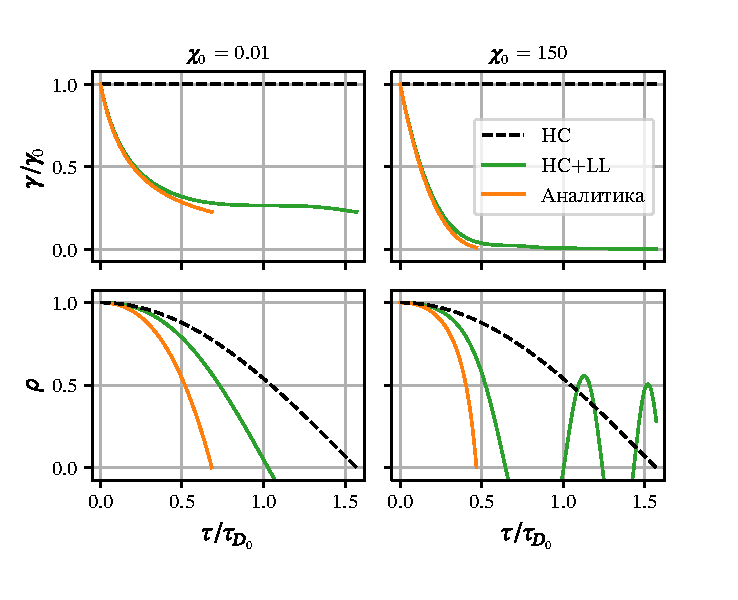
\includegraphics{beam-motionless.pdf}}
    \caption[Сравнение аналитического и численного решений уравнений движения частиц при столкновении пучков в режиме преобладания излучения]{\label{fig:ch3/sec2/motionless} 
    Сравнение приближённого решения~\eqref{eq:ch3/gamma_const}--\eqref{eq:ch3/rho_const} (оранжевая линия) с численным решением уравнений~\eqref{eq:ch3/dydt}--\eqref{eq:ch3/dgdt} (зелёная линия) при $\varkappa_0=5$. Для левой колонки $\chi_0=0.01$, для правой~---~$\chi_0=150$. Чёрная пунктирная линия соответствует решению уравнения~\eqref{eq:ch3/dydt} с постоянной энергией частицы $\gamma$.}
\end{figure}

\paragraph{Поправки модели}

Точность аналитической модели можно значительно повысить за счет двух изменений.
Во-первых, будем использовать среднюю поперечную координату в правой части уравнения~\eqref{eq:ch3/dydt} вместо ее начального значения $\rho_0$,
\begin{align}
    &\frac{d^2\rho}{d\tau^2} = -\frac{\mu}{\gamma} , \\
    \label{rho2}
    &\frac{d\gamma}{d\tau} = -P \left( \mu \chi_0 \frac{\gamma}{\gamma_0} \right), \\
    &\mu \equiv \frac{1}{\tau_D} \int^{\tau_D}_{0} \rho \left( \tau' \right) \dd \tau' < 1. 
\end{align}
Во-вторых, <<сошьём>> решения в КЭД и классическом режимах в момент времени $\tau_1$, при котором параметр частицы $\chi$ достигает некоторого порогового значения $\chi_1 \sim 1$, если его начальное значение было достаточно велико, то есть $\chi_0 > \chi_1$.
Тогда при $\tau < \tau_1$ уравнения движения имеют следующее решение
\begin{align}
    \label{eq:ch3/gamma_Q}
    &\gamma_Q(\tau) = \gamma_0 \left(1 - \tilde\varkappa_0 \frac{\tau}{\tau_{D_0}} \right)^{3} ,\\
    \label{eq:ch3/rho_Q}
    &\rho_Q(\tau) = 1 - \frac{\tau^2}{\tau_{D_0}^2}\left( 1-\tilde\varkappa_0 \frac{\tau}{\tau_{D_0}} \right)^{-1}, \\
    &\tilde\varkappa_0 = \sqrt{\frac{2}{9\gamma_0\mu}}P_Q(\mu\chi_0).
\end{align}
Отметим, что переменная $\tilde\varkappa_0$ (а также $\tilde\varkappa_1$ ниже) включает дополнительный множитель $1/3$ по сравнению с определением $\varkappa$ в уравнении~\eqref{eq:ch3/condition}, что несколько сокращает последующие выражения.
Момент времени $\tau_1$ находится из условия
\begin{align}
    \label{eq:ch3/chi1}
    \chi = \chi_0 \frac{\gamma_Q(\tau_1) \rho_Q(\tau_1)}{\gamma_0 } \equiv \chi_0 \frac{\gamma_1 \rho_1}{\gamma_0 } = \chi_1.
\end{align}
Для нахождения приближённого решения этого уравнения рассмотрим следующее вспомогательное уравнение относительно $x$
\begin{equation}
    \label{app.zeta}
    k_1 = \left( 1 - \frac{x^2}{1 - k_2 x} \right) \left( 1 - k_2 x \right)^3 .
\end{equation}
Поскольку оба множителя в правой части убывают с ростом $x$, очевидно, что $x < x_{1,2}$, где $x_{1,2}$ удовлетворяют следующим уравнениям
\begin{align}
    &k_1 = {\left(1 - k_2 x_1\right)}^3 ,\\
    &k_1 = 1 - \frac{x_2^2}{1 - k_2 x_2}.
\end{align}
Эти уравнения имеют следующие решения
\begin{align}
    &x_1 = \frac{1-\sqrt[3]{k_1}}{k_2}, \\
    &x_2 = \frac{k_2(1-k_1)}{2} \left( \sqrt{1 + \frac{4}{k_2^2 (1-k_1)}} - 1 \right).
\end{align}
Таким образом, приближенное решение уравнения ~\eqref{app.zeta} может быть найдено как $x = \text{min}\{x_1, x_2\}$.
Наконец $\tau_1$ находится путём выполнения замены
\begin{equation}
    x \rightarrow \frac{\tau_1}{\tau_{D_0}} ,\ 
    k_1 \rightarrow \frac{\chi_1}{\chi_0} = \zeta ,\ 
    k_2 \rightarrow \tilde{\varkappa}_0.
\end{equation}
Из уравнения~\eqref{eq:ch3/chi1} отношение $\gamma_1/\gamma_0$ можно найти следующим образом
\begin{equation}
    \frac{\gamma_1}{\gamma_0} = \frac{\chi_1}{\chi_0} \frac{1}{\rho_1} \equiv \frac{\zeta}{\rho_1},
\end{equation}
где мы ввели $\zeta=\chi_1/\chi_0$.

\begin{figure}
    \centerfloat{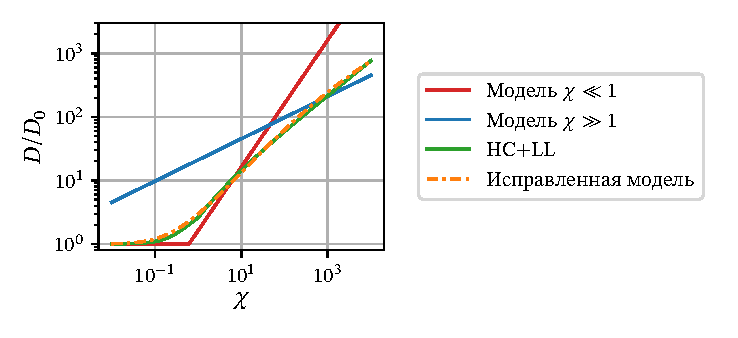
\includegraphics{beam-scalings.pdf}}
    \caption[Сравнение точности вычисления отношения $D/D_0$ в помощью различных методов]{\label{fig:ch3/scalings} 
    Сравнение отношения $D/D_0$, рассчитанного с помощью предельного выражения~\eqref{eq:ch3/dratio_simple} (красная линия соответствует классическому пределу, синяя~---~квантовому), с помощью исправленной модели (оранжевая штрих-пунктирная линия) и с помощью численного решения уравнений движения~\eqref{eq:ch3/dydt}--\eqref{eq:ch3/dgdt} (зелёная линия), как функция $\chi$ при фиксированном значении $r_\mathrm{b} = \SI{10}{\um}$.}
\end{figure}

При $\tau > \tau_1$ по определению необходимо использовать классические формулы для мощности излучения, так что решение уравнений движения имеет вид
\begin{gather}
    \label{eq:ch3/gamma_C}
    \gamma_C(\tau) = \gamma_1 \left(1+ 3\tilde\varkappa_1\frac{\tau - \tau_1}{\tau_{D_1}} \right)^{-1} ,\\
    \label{eq:ch3/rho_C}
    \rho_C(\tau) = \rho_1 + \dot{\rho}_1 \frac{\tau - \tau_1}{\tau_{D_1}} - \frac{(\tau-\tau_1)^2}{\tau_{D_1}^2}\left(1+\tilde\varkappa_1\frac{\tau - \tau_1 }{\tau_{D_1}}\right), 
\end{gather}
где
\begin{gather}
    \tau_{D_1}  = \sqrt{2 \gamma_1}, \\
    \tilde\varkappa_1 = \sqrt{\frac{2}{9\gamma_1\mu}}P_C(\mu\chi_1) , \\
    \dot{\rho}_1 = \tau_{D_1} \dot{\rho}_Q (\tau = \tau_1) = - \sqrt{\frac{\zeta}{\rho_1}}\frac{\tau_1 }{\tau_{D_0}}\frac{2-\tilde\varkappa_0 \frac{\tau_1}{\tau_{D_0}}}{\left( 1 - \tilde\varkappa_0 \frac{\tau_1}{\tau_{D_0}} \right)^2}. 
\end{gather}
Время фокусировки можно вычислить из уравнения $\rho_C(\tau_D) = 0$, имеющее явное, однако слишком громоздкое решение.
Найдём приближенное решение этого уравнения.
Для этого рассмотрим следующее вспомогательное уравнение относительно $x$
\begin{equation}
    \label{app.rho}
    0 = k_1 + k_2 x - x^2 \left( 1 + k_3 x \right).
\end{equation}
При больших значениях $k_3$ решения этого уравнения можно грубо оценить следующим образом
\begin{equation}
    x_1 = \sqrt[3]{\frac{k_1}{k_3}}.
\end{equation}
Для меньших значений $k_3$ мы можем сначала найти решение, положив $k_3=0$, т.е.
\begin{equation}
    0 = k_1 + k_2 x' - x'^2.
\end{equation}
Приведенное выше уравнение имеет решение
\begin{equation}
    x' = \frac{k_2}{2} + \sqrt{k_1 + \frac{k_2^2}{4}} .
\end{equation}
Предполагая, что решение уравнения ~\eqref{app.rho} лишь немного отличается от $x'$, т. е. $x=x'+x''$, мы можем разложить это уравнение по $x''$ и оставить только линейные члены:
\begin{equation}
    k_2 x'' + 2 x'' x' (1 + k_3 x') - k_3 x'^3 = 0.
\end{equation}
Отсюда получаем, что $x$ можно приближённо вычислить следующим образом
\begin{equation}
    x_2 = x' - \frac{k_3 x'^3}{k_2 + 2 x' (1 + k_3 x')}.
\end{equation}
Наконец, выбирается наименьшее из $x_{1,2}$, т.е.~$x~=~\text{min}\{x_1, x_2\}$.
Чтобы найти $\tau_2$, выполним следующую замену
\begin{equation}
    x \rightarrow \frac{\tau_2}{\tau_{D_1}} ,\ 
    k_1 \rightarrow \rho_1 ,\ 
    k_2 \rightarrow \dot{\rho}_1 ,\ 
    k_3 \rightarrow \tilde{\varkappa}_1. 
\end{equation}
Таким образом, 
\begin{gather}
    \label{eq:ch3/est0}
    \frac{\tau_D}{\tau_{D_0}} = \tau_1 + \tau_2 \sqrt{\frac{\zeta}{\rho_1}} ,\\
    \label{eq:ch3/est1}
    \tau_1 = \text{min}\left \{ \frac{1 - \zeta ^{1/3}}{\tilde\varkappa_0} \frac{\tilde\varkappa_0 \left( 1 - \zeta \right)}{2}  \left( \sqrt{1 + \frac{4}{\tilde\varkappa_0^2 \left( 1 - \zeta \right)}} - 1 \right) \right \}, \\
    \label{eq:ch3/est2}
    \tau_2 = \text{min}\left\{ \sqrt[3]{\frac{\rho_1}{\tilde\varkappa_1}}, \tau' - \frac{\tilde\varkappa_1 \tau'^3}{\dot\rho_1 + 2\tau' \left( 1 + \tilde\varkappa_1 \tau' \right)} \right\} ,\\
    \tau' = \sqrt{\rho_1 + \frac{\dot\rho_1^2}{4}} - \frac{\dot\rho_1}{2}.
\end{gather}
В случае $\chi_0 < \chi_1$, $\tau_1 \equiv 0$ и $\chi_1$ необходимо заменить на $\chi_0$ в $\tau_2$.

По аналогии с уравнением~\eqref{eq:ch3/beta0} параметр, определяющий значимость излучения, может быть выражен следующим образом
\begin{equation}
    \tilde\varkappa = \alpha \sqrt{ \frac{2}{9} r_\mathrm{b} a_\mathrm{S}} \times
    \begin{dcases}
        {\left( \mu\chi_0 \right)}^{2/3} ,\; \chi_0 < \chi_1, \\
        {\left( \mu\chi_0 \right)}^{1/6} ,\; \chi_0 > \chi_1,
    \end{dcases}
\end{equation}
и несложно показать, что $\tilde\varkappa_1$ можно выразить через $\tilde\varkappa$.
Таким образом, параметр разрушения с учётом реакции излучения в скорректированной модели равен
\begin{equation}
    D = {D_0} \left(\frac{\tau_{D_0}}{\tau_D}\right)^2.
\end{equation}
Рисунок~\ref{fig:ch3/scalings} показывает, что расчет параметра разрушения с использованием этой скорректированной модели значительно превосходит использование простых предельных выражений~\eqref{eq:ch3/dratio_simple}.
Заметим, что хотя $\mu$ следует вычислять самосогласованным образом из полученного выше решения, численный анализ показывает, что значение $\mu$ близко к $0.5$.
Таким образом, чтобы найти аналитическое решение, мы рассматриваем $\mu$ как свободный параметр, который мы устанавливаем равным $0.5$.
Это также подтверждается тем, что варьирование $\mu$ в диапазоне 0.3--0.7 не приводит к существенному изменению конечного значения параметра разрушения.
Согласно уравнениям~\eqref{eq:ch3/est1}--\eqref{eq:ch3/est2}, отношение $D/D_0$ может быть выражено как функция только от двух начальных параметров: радиуса пучка $r_\mathrm{b}$ и значения $\chi_0$.
Данный факт позволяет провести за разумное время сканирование по параметрам с помощью полноразмерного трёхмерного QED-PIC моделирования и вычислить значение $D/D_0$, основываясь на результатах такого моделирования (см. п.~\ref{sec:ch3/sec/PIC}).

\subsection{Взаимодействие длинных пучков}
\label{sub:ch3/sec3/Long}

В данном разделе обсуждается взаимодействие длинных однородных пучков противоположно заряженных частиц, когда число бетатронных колебаний велико $\sigma_z / (c \tau_{D_0}) \gg 1$ и радиационные потери на излучение незначительны в течение одного периода, что соответствует пределу $\varkappa \ll 1$.
Такая конфигурация может соответствовать взаимодействию пучков с существенно различающимися плотностями энергии в системе центра масс, что может возникать из-за большей массы, Лоренц-фактора или плотности частиц одного пучка по сравнению с другим в лабораторной системе отсчета.
Характерным примером такого сценария является столкновении электронного и протонного пучков.
В таком случае характерный временной масштаб эволюции более энергичного пучка намного больше, чем у встречного, поэтому все частицы встречного пучка ощущают практически невозмущенное поле в отличие от случая, рассмотренного в предыдущем разделе, когда данное утверждение верно только для частиц на фронте пучка.
Для простоты рассмотрим взаимодействие однородных пучков $\eta_z =\eta_r =\eta = 1$, для которых $\mathcal{E}(\rho) = \rho$.
Удобно ввести следующие переменные
\begin{gather}
    \label{b}
    a^{2} = \rho^{2}+\gamma\left(\dv{\rho}{\tau}\right)^2,\\
    \varphi = \arctan(\dv{\rho}{\tau}\frac{\sqrt{\gamma}}{\rho}) ,
\end{gather}
где $a$ и $\varphi$~---~амплитуда и фаза бетатронных колебаний ($\rho = a \cos\varphi $).
В новых переменных уравнение~\eqref{eq:ch3/app_g} принимает вид
\begin{equation}
    \label{rho}
    \dv{a}{\tau} = -\frac{a}{2\gamma}\sin^{2}\varphi\;P\left( \frac{\chi_0}{\gamma_0} a \gamma  |{\cos\varphi} | \right).
\end{equation}
Чтобы вычислить медленно меняющуюся амплитуду бетатронных колебаний, $A = \left\langle a\right\rangle $, усредним уравнение~\eqref{rho} по $\varphi$ и пренебрежём быстрыми составляющими амплитуды $a$ и энергии $\gamma$
\begin{gather}
    \label{dst-2}
    \dv{A}{\tau} = -\frac{A}{2\overline{\gamma}}f_{1}\left(\frac{\chi_0}{\gamma_0} A \overline{\gamma} \right),\\
    \dv{\overline{\gamma}}{\tau} = -f_{2}\left(\frac{\chi_0}{\gamma_0} A \overline{\gamma} \right),\\
\end{gather}
где 
\begin{gather}
    \label{f1}
    f_{1}(v) = \frac{1}{2\pi}\intop_{0}^{2\pi}\sin^{2}\varphi\;P\left(v|{\cos\varphi} |\right)\dd\varphi ,\\
    f_{2}(v) = \frac{1}{2\pi}\intop_{0}^{2\pi}P\left(v |{\cos\varphi}|\right)\dd\varphi ,
\end{gather}
и $\overline{\gamma} = \langle\gamma\rangle$.
Вводя $\overline{\chi}=\left\langle \chi\right\rangle = \chi_0 A \overline{\gamma} / \gamma_0$, получаем систему, описывающую усредненную по бетатронным колебаниям динамику электрона
\begin{gather}
    \label{v}
    \frac{d\overline{\chi}}{d\tau} = -\frac{\overline{\chi}}{2\overline{\gamma}}\left[f_{1}\left(\overline{\chi}\right)+2f_{2}\left(\overline{\chi} \right)\right],\\
    \label{gf2}
    \frac{d\overline{\gamma}}{d\tau} = -f_{2}\left(\overline{\chi } \right).
\end{gather}
Данная система имеет следующий интеграл движения
\begin{gather}
    \ln \overline{\gamma} - g (\overline{\chi} )  = \mathrm{const} \label{integral} , \\
    g (v) = \int \frac{2f_{2}(v)\dd v} {v f_{1}\left(v \right)+2 v f_{2}\left(v \right)}.
\end{gather}
\begin{figure}[ht]
	\centerfloat{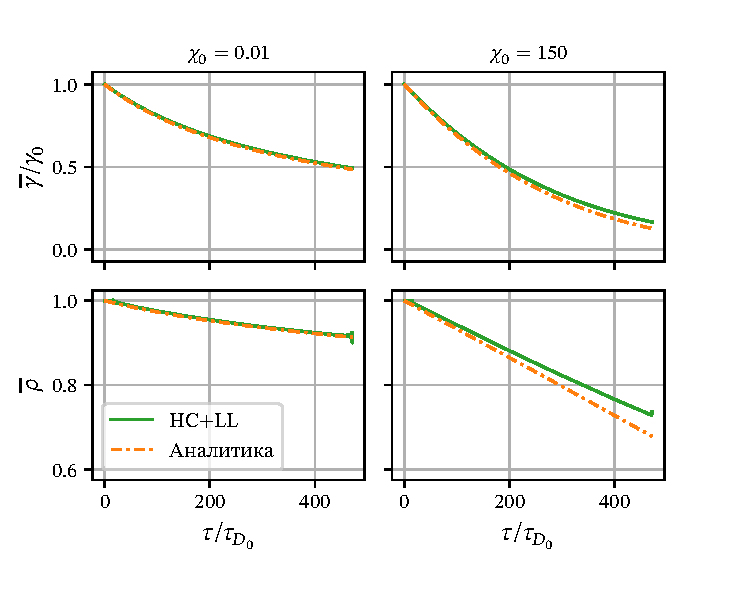
\includegraphics{beam-long.pdf}}
	\caption[Сравнение аналитического и численного решений уравнений движения частиц при столкновении длинных пучков в режиме слабого пучкового излучения]{\label{fig:ch3/sec3/long} 
    Сравнение аналитического решения~\eqref{eq:ch3/long_gC}--\eqref{eq:ch3/long_rC} и~\eqref{eq:ch3/long_gQ}--\eqref{eq:ch3/long_rQ} (оранжевая штрих-пунктирная линия) и численного решения уравнений~\eqref{eq:ch3/dydt}--\eqref{eq:ch3/dgdt} (зелёная линия) при $\varkappa_0=0.005$. В левой колонке $\chi_0=0.01$, в правой~---~$\chi_0=150$.}
	\label{long}
\end{figure}
В классическом пределе ($\chi \ll 1$) $f_{2}(v) = 4 f_{1}(v)=P_C(v)/2$ и интеграл движения принимает вид
\begin{equation}
    \overline{\gamma}^{-9/8} \overline{\chi} = \text{const}.\label{integral1}
\end{equation}
Из уравнений~\eqref{gf2} и \eqref{integral1} следует, что
\begin{gather}
    \label{eq:ch3/long_gC}
    \overline{\gamma} = \gamma_{0} S(\tau)^{-4/5} ,\\
    \label{eq:ch3/long_rC}
    \overline \rho = \rho_{0} S(\tau)^{-1/10},\\
    % & \overline{\chi} = \chi_{0} S(\tau)^{-9/10}, \\
    S(\tau) = 1+\frac{5}{8}\left( \varkappa\frac{\tau}{\tau_{D_0}} \right).
\end{gather}
% Fig.~\ref{long1} demonstrates numerical solution of Eqs.~\eqref{eq:ch3/y2}-\eqref{eq:ch3/c2}
% and analytical result  given by Eq.~\eqref{eq:ch3/long_gC} for $\ln\gamma(t)$ which are in a good agreement.
В существенно квантовом пределе (${\chi\gg1}$)
\begin{equation}
    f_{2}(v)= (8/3) f_1 (v) = \Gamma(5/6) \Gamma^{-1}(4 /3) \pi^{-1/2} P_Q(v),
\end{equation} 
и интеграл движения принимает вид
\begin{equation}
    \overline{\gamma}^{-19/16}\overline{\chi} = \text{const}.\label{integral1-1}
\end{equation}
Уравнения~\eqref{gf2} и \eqref{integral1-1} имеют следующие решения
\begin{gather}
    \label{eq:ch3/long_gQ}
    \overline{\gamma} = \gamma_{0} S(\tau)^{24/5},\\
    \label{eq:ch3/long_rQ}
    \overline\rho  = \rho_{0} S(\tau)^{9/5},\\
    % &\overline{\chi} = \chi_{0} S(\tau)^{57/10}, \\
    S(\tau) = 1-\frac{5}{24\sqrt\pi}\frac{\Gamma(5/6)}{\Gamma(4/3)}\left( \varkappa\frac{\tau}{\tau_{D_0}} \right) \approx 1 - 0.149\left( \varkappa\frac{\tau}{\tau_{D_0}} \right).
\end{gather}
Рисунок~\ref{fig:ch3/sec3/long} демонстрирует хорошее совпадение численного решения уравнений~\eqref{eq:ch3/dydt}--\eqref{eq:ch3/c2} и аналитического решения~\eqref{eq:ch3/long_gC} и~\eqref{eq:ch3/long_gQ}.

\subsection{QED-PIC моделирование}
\label{sec:ch3/sec/PIC}

Для подтверждения предсказаний модели, разработанной в п.~\ref{sub:ch3/sec3/Model} было выполнено полноразмерное трехмерное QED-PIC моделирование с использованием кода QUILL~\cite{QUILL}, который позволяет моделировать КЭД процессы с учётом их стохастичности с помощью метода Монте-Карло.
Принимая $z$ за ось распространения пучка, параметры моделирования составляли $\Delta t = 0,6 \Delta z$, $\Delta x = \Delta y = 2,5 \Delta z = r_\mathrm{b} / 20$.
Для всех проведенных моделирований шаг по времени $\Delta t$ был намного меньше, чем средняя задержка между последовательными КЭД процессами (излучением гамма-кванта или рождения электрон-позитронной пары).
Для численного решения уравнений Максвелла использовалась гибридная схема FDTD, подробно опиаснная в разделе~\ref{sub:ch3/sec4/Hybrid}, а для решения уравнений движения частиц использовался пушер Вэя~\cite{Vay08}.
Моделирование также выполнялось с использованием кода VLPL~\cite{pukhov1999three,NDFX,PhysRevE_94_063204} в сочетании с бездисперсионной схемой решения уравнений Максвелла~---~RIP~\cite{Pukhov2019}.
Различия между результатами моделирования с использованием двух разных кодов были незначительными.
На рисунке~\ref{fig:ch3/densities}, демонстрирующем пример результатов моделирования, видно, что при $\chi_0 = 10$ происходит обильное рождение вторичных электронов и позитронов.
Поскольку этот процесс не влияет на движение частиц пучка на фронте, формирование и развитие такого каскада подробно не обсуждается.
Также отметим развитие поперечной шланговой неустойчивости в моделировании с учетом КЭД процессов, которая будет описана ниже.

\begin{figure}[ht]
    \centerfloat{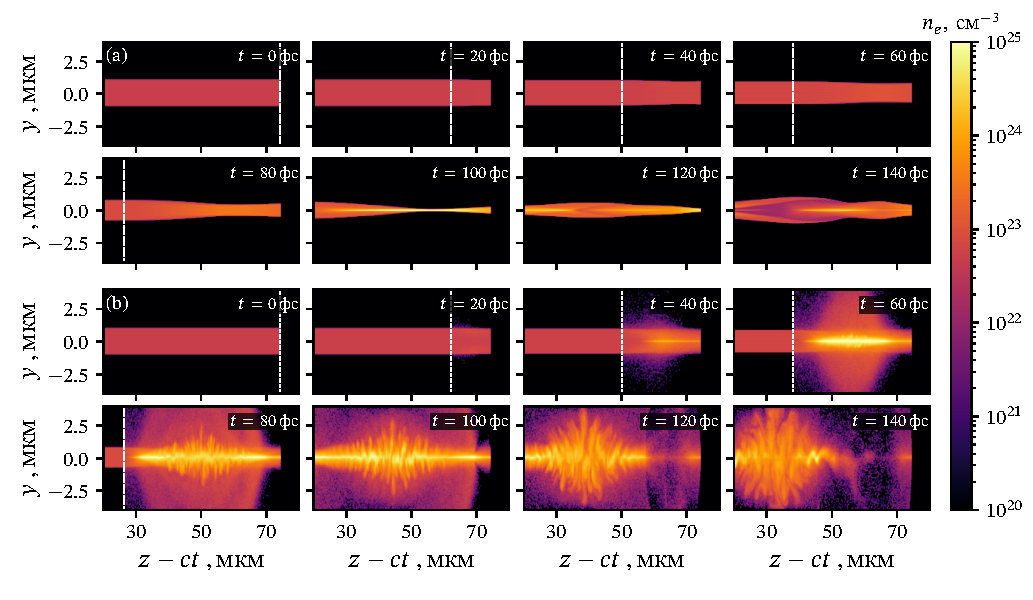
\includegraphics{beam-density.pdf}}
    \caption[Распределение плотности электронов в различные моменты времени в PIC моделировании столкновения электронного и позитронного пучков]{\label{fig:ch3/densities} 
    Распределение плотности электронов в различные моменты времени в PIC моделировании с параметрами $r = \SI{1}{\um}$, $\chi = 10$. 
    Белая пунктирная линия соответствует положению фронта встречного позитронного пучка.
    Представлены результаты моделирования (a) без учёта и (b) с учётом КЭД процессов.}
\end{figure}

Мы провели серию моделирований с различными значениями начального радиуса пучков $r_\mathrm{b}$ и величины $\chi_0$.
Длина пучка выбиралась таким образом, чтобы для каждого моделирования параметр разрушения без учёта реакции излучения, т.е. $D_0$, равнялся 10.
Это было сделано для того, чтобы иметь четкий способ определения времени фокусировки, используемого при расчете параметра разрушения.
В этом отношении наше QED-PIC моделирование не соответствует какому-либо конкретному эксперименту, возможному, например, на установке FACET-II, поскольку последний требует очень короткого времени взаимодействия для подавления радиационных потерь~\cite{yakimenko2019prospect}.
Вместо этого QED-PIC моделирование использовалось как средство для решения уравнений движения частиц в самосогласованно вычисляемом электромагнитном поле и с учетом стохастического характера КЭД процессов.
Для каждого моделирования мы отслеживали несколько сотен частиц, расположенных на фронте и периферии электронного пучка, по траекториям которых рассчитывалось среднее время пересечения оси пучка.
Примеры таких траекторий, численное решение уравнений~\eqref{eq:ch3/dydt}--\eqref{eq:ch3/dgdt} и приближенное аналитическое решение показаны на Рис.~\ref{fig:ch3/tracks}.
Для каждой пары значений $r_\mathrm{b}$ и $\chi_0$ проводилось два моделирования: с учётом и без КЭД процессов.
Сравнивая среднее время фокусировки в этих двух моделированиях, рассчитывалось отношение $D/D_0$ в широком диапазоне начальных параметров, что представлено на Рис.~\ref{fig:ch3/disruption} вместе с оценкой из уравнений~\eqref{eq:ch3/est0}-- \eqref{eq:ch3/est2} (в котором были использованы свободные параметры $\mu=0.5$, $\chi_1=1$) и результатом численного решения одночастичных уравнений движения~\eqref{eq:ch3/dydt}- -\eqref{eq:ch3/dgdt}.

\begin{figure}[ht]
    \centerfloat{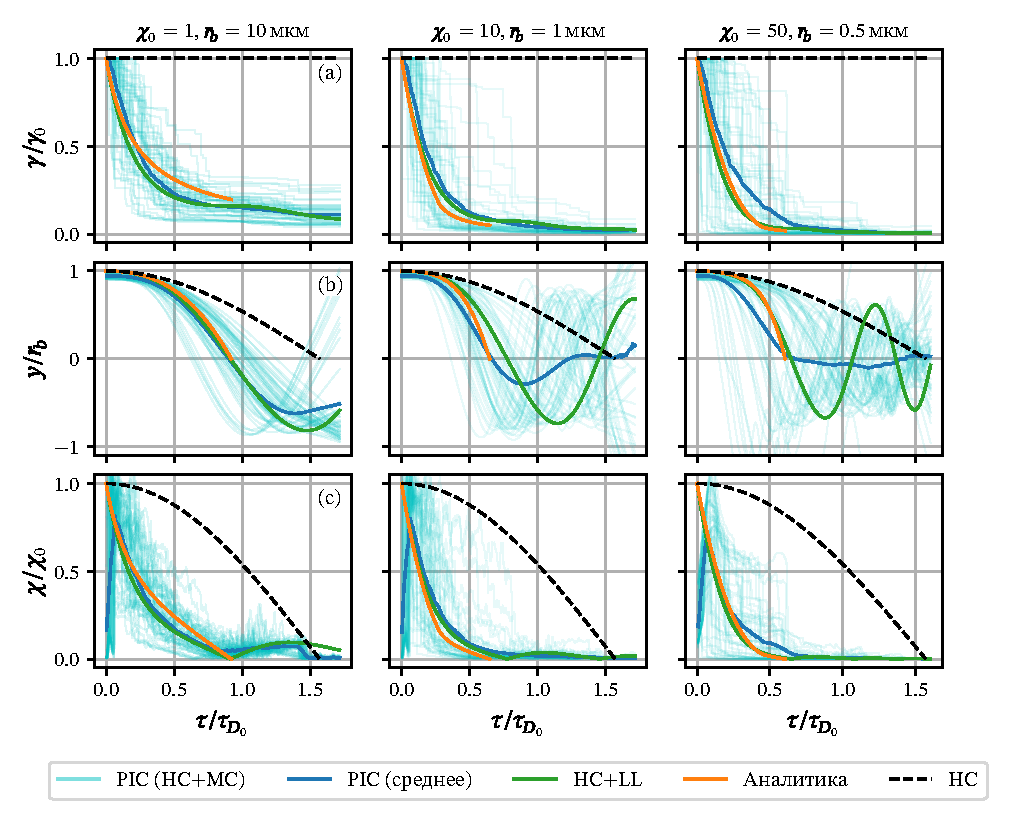
\includegraphics{beam-tracks.pdf}}
    \caption[Динамика электронов в поле встречного позитронного пучка]{\label{fig:ch3/tracks} 
    Динамика электронов в поле встречного позитронного пучка. (a) Энергия электронов, (b) смещение относительно оси пучка и (c) величина параметра $\chi$ как функции времени.
    Тонкие голубые линии соответствуют траекториям отдельных частиц в QED-PIC моделировании, сплошная синяя линия~---~величинам, усреднённым по этим частицам, зелёная линия~---~численному решению уравнений~\eqref{eq:ch3/dydt}--\eqref{eq:ch3/dgdt}, оранжевая линия~---~аналитическому решению ~\eqref{eq:ch3/gamma_Q}--\eqref{eq:ch3/rho_Q},~\eqref{eq:ch3/gamma_C}--\eqref{eq:ch3/rho_C}, чёрная пунктирная линия~---~решению уравнения~\eqref{eq:ch3/dydt} без учёта пучкового излучения, т.е. с постоянной энергией $\gamma$.
    Различные колонки соответствуют различным начальным параметрам $r_\mathrm{b}$ и $\chi_0$.}
\end{figure}

\begin{figure}[ht]
    \centerfloat{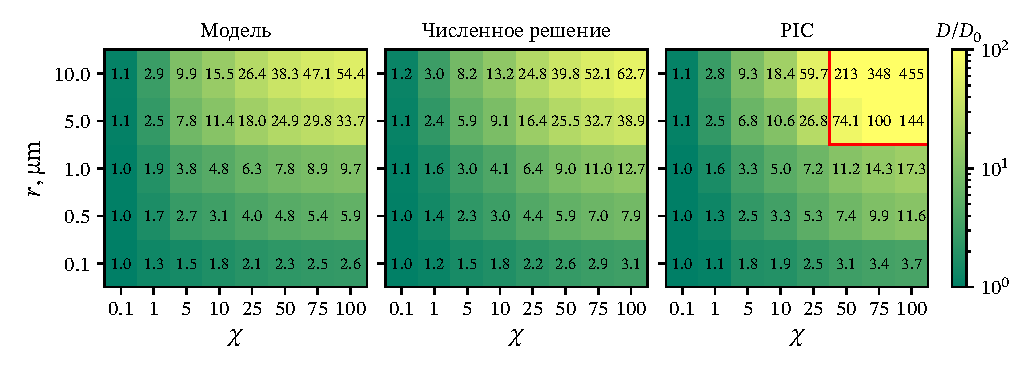
\includegraphics{beam-map.pdf}}
    \caption[Сравнение отношения параметра разрушения с учётом реакции излучения к таковому без учёта реакции излучения, рассчитанного различными способами]{\label{fig:ch3/disruption} 
    Отношение $D/ D_0$, рассчитанное (левая колонка) по аналитическому решению~\eqref{eq:ch3/est0}--\eqref{eq:ch3/est1}, (средняя колонка) по численному решению уравнений~\eqref{eq:ch3/dydt}--\eqref{eq:ch3/dgdt}, (правая колонка) полученная по результатам QED-PIC моделирования.
    Красная рамка обозначает область, в которой был использован альтернативный критерий разрушения (см. текст).}
\end{figure}

Важно отметить, что для больших значений $r_\mathrm{b}$ и $\chi_0$ (область, отмеченная красной рамкой на Рис.~\ref{fig:ch3/disruption}) для расчета параметра разрушения был использован альтернативный критерий.
Это связано с тем, что при таких параметрах потери энергии из-за излучения настолько велики, что через некоторое время частицы пучка перестают быть релятивистскими, а их продольная скорость становится сравнимой с их поперечной скоростью, так что в конце концов частицы прекращают свое направленное движение и начинают вращение, не пересекая ось луча (\fixme{рисунок с треками}).
В таких случаях для вычисления параметра разрушения вместо времени достижения частицей оси пучка, использовалось время, за которое продольная скорость частицы достигала значения $0.5c$.
Поскольку наша аналитическая модель предполагает, что продольная скорость всегда больше поперечной, она не может быть применена в этих случаях.
% Изучение столкновений пучков в этой области параметров требует отдельного специального исследования.
Как было указано выше, наша аналитическая модель предсказывает, что отношение $D/D_0$ не зависит явно от энергии частиц.
Для подтверждения этого нами было выполнено несколько QED-PIC моделирований с разными начальными энергиями частиц, но с одинаковыми значениями $\chi_0$ и $r_\mathrm{b}$.
Результаты моделирования показывают, что до тех пор, пока энергия частицы достаточно велика, для того чтобы частицы оставались ультрарелятивистскими до достижения оси пучка, результирующее отношение $D/D_0$ не зависит от энергии частицы.

\fixme{Мы не проводили QED-PIC-симуляции взаимодействия пучков в режиме, когда лучевое излучение требует много бетатронных колебаний для значительного уменьшения энергии частиц ($\varkappa \ll 1$) по нескольким причинам.
Во-первых, такие симуляции заняли бы значительно больше времени.
А во-вторых, поскольку этот режим в большей степени связан с взаимодействием пучков с существенно различающимися плотностями энергии (в системе центра масс), при котором более энергичный из них сильно не деформируется, такое взаимодействие может быть достаточно смоделировано одной частицей динамики в невозмущенном поле медленно эволюционирующего (энергетического) сгустка, что было сделано в разд.~\ref{sub:ch3/sec3/Model}.}

\subsection{Обсуждение}
\label{sec:ch3/sec/Discussion}

Схема, обсуждаемая в публикации~\cite{yakimenko2019prospect}, для наблюдения эффектов непертурбативной КЭД с помощью лобового столкновения электронного и позитронного пучков, требует столкновения пучков очень малому параметру разрушения.
Это требование накладывает жесткие ограничения на длину и диаметр пучка.
Однако, как показано выше на параметр разрушения также влияет реакция излучения, которая не учитывается при стандартном способе расчёта параметра разрушения.
Наша аналитическая модель показывает, что при параметрах пучка, необходимых для достижения значения $\chi \sim 1600$ при энергии пучка $\SI{125}{\giga\electronvolt}$, полном заряде $\SI{3}{\nano\coulomb}$ и радиусе $\SI{10}{\nano\meter}$, увеличение разрушения из-за излучения достигает 60\%.
Для будущих коллайдеров CLIC и ILC, наоборот, реакция излучения может несколько смягчить требования к параметрам пучка для достижения желаемой яркости в области взаимодействия, что частично достигается за счет использования плоских пучков.
Хотя при выводе аналитической оценки отношения $D/D_0$ мы рассматривали цилиндрические пучки, полученные результаты можно применить к конфигурациям плоских пучков, предлагаемых для использования на установках CLIC и ILC.
Для частиц, с начальным отклонением, лежащим на одной из осей пучка, движение остается плоским, и поэтому уравнения ~\eqref{eq:ch3/dydt}--\eqref{eq:ch3/dgdt} остаются справедливыми.
Таким образом, вычисляя значения $\chi_0$ и $r_\mathrm{b}$ относительно распределения заряда пучка (см., например,~\cite{bassetti1983properties} для распределения электромагнитных полей для эллиптического гауссова распределения заряда), параметр разрушения может быть вычислен для конкретной оси с использованием нашей аналитической модели.
Выполнение этой процедуры, приводит к заключению, что для ожидаемых параметров пучка на установке CLIC увеличение параметра разрушения составляет примерно $35\%$ для более длинной оси и только на $5\%$ для более короткой.
Для круглого пучка с тем же полным зарядом и площадью поперечного сечения увеличение параметра разрушения составляет около $35\%$ по обеим осям, что  подтверждает тот факт, что использование плоских пучков снижает влияние реакции излучения на столкновение пучков.
Для параметров, ожидаемых на установке ILC, увеличение разрушения не превышает $5\%$ по обеим осям из-за достаточно низкого значения $\chi$.

\begin{figure}[ht]
    \centerfloat{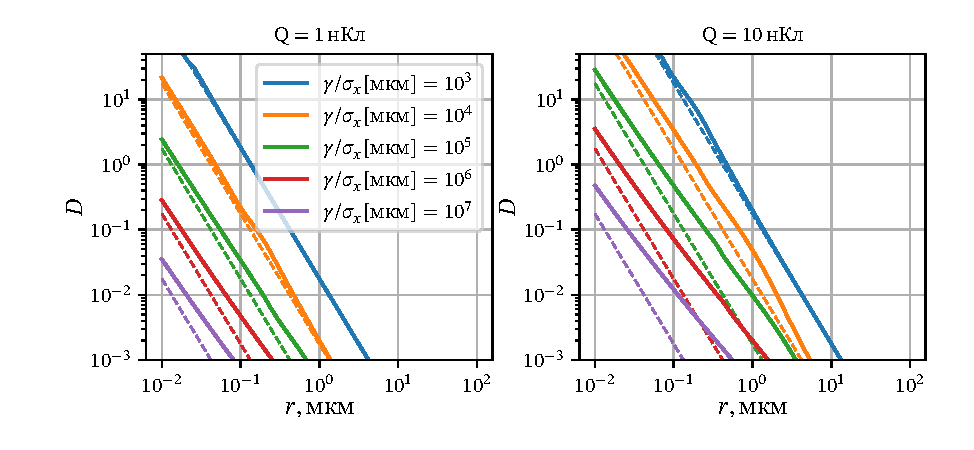
\includegraphics{beam-Q_disruption.pdf}}
    \caption[Параметр разрушения, рассчитанный с учётом и без учёта пучкового излучения, для различных параметров пучка]{\label{fig:ch3/Q_disruption} 
    Параметр разрушения, рассчитанный с учётом (сплошные линии) и без учёта (пунктирные линии) пучкового излучения, для различных параметров пучка.}
\end{figure}

На Рис.~\ref{fig:ch3/Q_disruption} показано, как реакция излучения влияет на разрушение пучков при различных параметрах.
В частности, показано, что столкновение пучков с достаточно большим полным зарядом ($> \SI{10}{\nano\coulomb}$ 10 нКл) и малыми радиусами может быть подвержено существенному влиянию пучкового излучения.
Другая интересная зависимость заключается в том, что хотя увеличение энергии частиц и/или уменьшение длины пучка (при сохранении того же общего заряда) уменьшает параметр разрушения, оно в то же время приводит к увеличению значимости пучкового излучения.
Таким образом, отношение $D/D_0$ можно использовать для определения того, является ли излучение при столкновении пучков значительными или нет.

\begin{comment}
    Динамика пучка при взаимодействии пучков с противоположными зарядами была исследована в режиме доминирования излучения.
    Оказывается, радиус пучка $r_\mathrm{b}$ и $\chi_0$ являются ключевыми параметрами, определяющими усиление фокусировки или разрушения пучков.
    Для однородного пучка параметр $\chi_0$ можно рассчитать по плотности пучка $n_e$ или полному заряду пучка $Q$ следующим образом
    \begin{equation}
        \chi_0 \approx 5.3\; \frac{\varepsilon_\mathrm{b}[100\,\text{GeV}]\ Q[\text{nC}]}{r_\mathrm{b}[\upmu \text{m}]\; \sigma_z [\upmu \text{m}]} 
            \approx  2.67\; \varepsilon_\mathrm{b}[100\,\text{GeV}]\; n_e[10^{21}\text{cm}^{-3}] \;r_\mathrm{b}[\upmu \text{m}],
    \end{equation}
    где $\varepsilon_\mathrm{b}$~---~энергия частиц пучка.
    Согласно нашей модели постоянной силы отношение параметра разрушения с учётом пучкового излучения к параметру разрушения без его учёта также может быть выражено через параметры пучка.
    В классическом режиме ($\chi_0 \ll 1$)
    \begin{equation}
        \begin{aligned}
            D &\approx 4\times 10^{-3} \frac{Q[\text{nC}]^2}{r_\mathrm{b}[\upmu \text{m}]^{8/3}} 
            &\approx 8\times 10^{-4} n_e[10^{21}\text{cm}^{-3}]^2\sigma_z [\upmu \text{m}]^2 r_\mathrm{b}[\upmu \text{m}]^{2/3},
        \end{aligned}
    \end{equation}
    \begin{equation}
        \begin{aligned}
            \frac{D}{D_0} &\approx  22.1\; \frac{\varepsilon_\mathrm{b} [100\,\text{GeV}]\; Q[\text{nC}]}{r_\mathrm{b}[\upmu \text{m}]^{2/3} \;\sigma_z [\upmu \text{m}]} \\
            &\approx 8.9\; \varepsilon_\mathrm{b} [100\,\text{GeV}] \;n_e[10^{21}\text{cm}^{-3}] \;r_\mathrm{b}[\upmu \text{m}]^{2/3},
        \end{aligned}
    \end{equation}
    и в квантовом режиме ($\chi_0 \gg 1$)
    \begin{equation}
        \begin{aligned}
            D &\approx 7.2\times 10^{-3}\left( \frac{Q[\text{nC}]^2 \sigma_z[\upmu \text{m}]}{\varepsilon_\mathrm{b}[100\,\text{GeV}] r_\mathrm{b}[\upmu \text{m}]^2} \right)^{2/3}    \\
            &\approx 1.4\times 10^{-3}\left( \frac{n_e[10^{21}\text{cm}^{-3}]^{2} \sigma_z[\upmu \text{m}]^3 }{\varepsilon_\mathrm{b} [100\,\text{GeV}] r_\mathrm{b}[\upmu \text{m}]^{-2}} \right)^{2/3} ,
        \end{aligned}
    \end{equation}
    \begin{equation}
        \begin{aligned}
            &\frac{D}{D_0} \approx 38.8\left(\frac{r_\mathrm{b}[\upmu \text{m}]^{2} \;\varepsilon_\mathrm{b}[100\,\text{GeV}] \;Q[\text{nC}]}{\sigma_z [\upmu \text{m}]}\right)^{1/3} \\
            &\approx 15.6\left( \varepsilon_\mathrm{b}[100\,\text{GeV}] \;n_e[10^{21}\text{cm}^{-3}] \;r_\mathrm{b}[\upmu \text{m}]^4 \right)^{1/3} .
        \end{aligned}
    \end{equation}
    В приведенных выше выражениях мы использовали следующее выражение для параметра разрушения без учёта пучкового излучения $D_0$
    \begin{equation}
        \begin{aligned}
            D_0 &\approx 1.8\times 10^{-4}\, \frac{Q[\text{nC}]\;\sigma_z[\upmu \text{m}]}{\varepsilon_\mathrm{b}[100\,\text{GeV}] \;r_\mathrm{b}[\upmu \text{m}]^2}, \\
            &\approx 0.9\times 10^{-4}\,\frac{n_e[10^{21}\text{cm}^{-3}] \;\sigma_z[\upmu \text{m}]^2}{\varepsilon_\mathrm{b}[100\,\text{GeV}]}.
        \end{aligned}
    \end{equation}
    Более точное значение $D$ можно рассчитать по скорректированной модели, представленной в п.~\ref{subsec:ch3/sec/Corrections}.
\end{comment}


\paragraph{Столкновение пучков одного знака}

Разработанная выше модель, описывающая увеличение параметра разрушения за счёт реакции излучения, может быть расширена и на случай столкновения пучков с одинаковым знаком заряда.
В таком случае параметр разрушения является квадратом отношения времени, за которое отклонение частиц от оси пучка увеличивается вдвое, к времени взаимодействия пучков.
Вычисление этого параметра с учётом реакции излучения может быть проведено с помощью аналогичного метода, который был использован выше, т.е. за счёт замены в правой части уравнений движения частиц мгновенного значения силы, действующей на частицу, на её среднее значение.
Так же как и в случае столкновения противоположно заряженных пучков, в данном случае поперечное отклонение частицы изменяется в ограниченном интервале от $r_0$ до $2r_0$, поэтому такое приближение обосновано.
Также данная процедура позволяет неявно учесть тот факт, что сила, действующая на частицу за пределами пучка, спадает по закону $1/r$.
Отметим, что при взаимодействии пучков одного знака частицы совершают инфинитное движение, а не осциллируют, поэтому оба режима взаимодействия, соответствующие столкновению либо коротких, либо длинных пучков, могут быть описаны нами одной аналитической моделью.
Таким образом, оказывается, что несмотря на различный характер движения частиц в случае столкновения одинаково или противоположно заряженных пучков, конечные формулы для вычисления параметра разрушения с учётом реакции излучения идентичны в обоих этих случаях.
Таким образом, область применимости предложенного нами способа вычисления параметра разрушения пучков с учётом реакции излучения распространяется и на случай взаимодействия пучков одного заряда. Отметим, что экспериментальная реализация столкновения, например, двух электронных пучков является более простой задачей, чем столкновение электронного и позитронного пучков, однако, например, с точки зрения достижения непертурбативного режима квантовой электродинамики такие конфигурации равнозначны.

\paragraph{\fixme{Изгибная неустойчивость (скопировано из отчёта РФФИ)}}

Помимо излучения частицами жёстких фотонов при столкновении сильноточных пучков, важным КЭД эффектом является распад излученных фотонов на вторичные электрон-позитронные пары.
Проведённое нами полноразмерное численное QED-PIC моделирование показывает, что в достаточно большом диапазоне начальных параметров (максимальное начальное значение параметра $\chi$ для частиц превышает 1) образующаяся таким образом электрон-позитронная плазма имеет существенно большую плотность, чем плотность начальных частиц.
В такой плазме за счёт небольшого пространственного разделения электронной и позитронной компонент экранируется электрическое поле начальных пучков.
Таким образом, задача о динамике вторичной плазмы может быть сведена к задаче о динамике нейтральных потоков во внешнем магнитном поле (начальных пучков), которая является одной из наиболее распространённых задач в астрофизике.
Известно, что в такой задаче может развиваться ряд неустойчивостей.
Численное моделирование показывает, что наиболее выраженной является шланговая неустойчивость плазменного потока в азимутальном магнитном поле, представляющая собой отклонение центра масс пучка от его средней оси симметрии.
Данный факт вероятно объясняется тем, что процесс фотообразования электрон-позитронных пар является стохастическим, поэтому даже при столкновении изначально цилиндрически-симметричных пучков образующаяся плазма не имеет такой симметрии.
При этом из-за каскадного образования вторичных электронов и позитронов возмущения плотности электрон-позитронной плазмы растут со временем.
Такие возмущения становятся затравкой для развития уже макроскопической шланговой неустойчивости.
Для оценки выхода вторичных частиц в процессе столкновения пучков можно воспользоваться известными формулами из публикаций~\cite{yokoya1992beam, chen1989coherent}, которые описывают рост числа фотонов и электрон-позитронных пар в зависимости от одного начального параметра - среднего значения chi частиц.
Отметим, что данными формулами можно пользоваться для оценки числа вторичных частиц первого “поколения”, т.е. в предположении, что образующиеся электроны и позитроны не излучают следующее “поколение” фотонов.
Данное предположение верно только для столкновения достаточно коротких пучков.
Численное моделирование показывает, что при достаточно продолжительном времени взаимодействия пучков в результате развития КЭД каскада могут образовываться вплоть до 10-100 поколений.
Оценка числа вторичных частиц в таком случае крайне затруднительна, так как вторичная плазма начинает оказывать обратное влияние на развитие каскада за счёт, например, экранировки электрического поля пучков, как это описано выше.

В публикации~\cite{filipovic2021effect} была изучена возможность существенного увеличения выхода вторичных частиц при столкновении сильноточных пучков за счёт относительного сдвига их осей.
При этом сдвиг определяется таким образом, чтобы ось одного пучка находилась в области максимального поля встречного пучка. Нами было показано что в такой конфигурации, несмотря на меньшую область геометрического перекрытия пучков, доля частиц, достигающих непертурбативного режима КЭД ($\alpha \chi^{2/3} > 1$), не отличается от таковой в несмещённой конфигурации.
При этом преимуществом смещённой конфигурации является более однородное распределение вторичных частиц, так как в таком случае все частицы пучка чувствуют примерно одинаковую напряжённость поля встречного пучка.
В случае несмещённой конфигурации максимальное поле чувствуют частицы на периферии пучка, что приводит к тому, что распределение вторичных частиц имеет форму кольца.
Численное моделирование также показывает увеличение выхода числа вторичных частиц в смещённой конфигурации вплоть до 5-10\%.
Аналогичный результат получается при вычислении числа вторичных частиц с помощью оценок, указанных выше.
Так как реализация такой конфигурации не требует никаких дополнительных усложнений с точки зрения эксперимента, очевидно её преимущество по сравнению с несмещённой конфигурацией.


В 2022 году было продолжено изучение изгибной неустойчивости, возникающей при лобовом столкновении сильноточных электронного и позитронного пучков.
Во-первых, было определено влияние вторичных электрон-позитронных пар, образующихся в результате распада жёстких фотонов, излученных начальными частицами пучка, на развитие данной неустойчивости.
Результаты полноразмерного трёхмерного QED-PIC моделирования показывают, что образование вторичных пар существенно не изменяет характерный пространственный масштаб неустойчивости и её инкремент.
Данный результат объясняется тем, что такие частицы не приводят к генерации как магнитных полей, т. к. суммарный ток образованной электрон-позитронной пары равен нулю, так и электростатических, т. к. они в среднем компенсируются за счёт симметричного образования пары из встречного пучка, создающих противоположное поле.
Таким образом вторичные электрон-позитронные пары создают квази-нейтральный фон достаточно большой плотности.
Результаты моделирования с искусственно отключенным образованием электрон-позитронных пар показывают, что затравка для шланговой неустойчивости создаётся в результате нарушения симметричности распределения заряда пучков, вызванного стохастическим излучением фотонов частицами пучка.
Последнее приводит к существенному уширению энергетического спектра пучка.
Так как частицы с меньшей энергией быстрее фокусируются в поле встречного пучка, это в конечном итоге приводит к тому, что распределение заряда в пучках приобретает случайную составляющую.

Во-вторых, были оценены характерный временной и пространственный масштабы наблюдаемой неустойчивости.
Для этого была модифицирована давно разработанная теорией её линейной стадии~\cite{chin1987stability, yokoya1992beam}.
Согласно этой теории эти масштабы по порядку величины совпадают с релятивистской плазменной частотой, соответствующей плотности пучка.
Важным отличием между исследуемой нами задачей и модельной задачей, с помощью которой описывается изгибная неустойчивость, заключается в том, что в последней предполагается постоянство энергии частиц и распределение собственных полей пучков.
Оба этих предположения оказываются неверными в рассматриваемой нами задаче.
Непостоянство энергии можно учесть с помощью теории, разработанной нами в 2020 году в рамках выполнения данного проекта, описывающей увеличение параметра разрушения пучков при учёте реакции излучения.
Так как релятивистская плазменная частота пропорциональна корню из параметра разрушения, то отношение характерной длины волны изгибной неустойчивости с учётом реакции излучения к таковой без учёта реакции равно корню из отношения соответствующих параметров разрушения, вычисляемого с помощью нашей теории.
Фокусировка и соответствующее увеличение плотности пучков приводит к дополнительному увеличению плазменной частоты.
В связи со стохастичностью излучения, максимальная концентрация сфокусированного пучка существенно меньше, чем в случае без учёта реакции излучения. Согласно результатам моделирования, отношение максимальной плотности пучка к начальной достигает значения порядка 10.
Таким образом для определения характерного масштаба изгибной неустойчивости с учётом реакции излучения можно рассчитать по стандартным формулам, а затем умножить результат на корень из произведения отношения максимальной плотности пучка к начальной и отношения параметра разрушения с учётом реакции излучения к таковому без учёта реакции излучения.
Вычисленный таким образом пространственный масштаб совпадает по порядку величины с результатами полноразмерного QED-PIC моделирования.
В-третьих, согласно той же линейной теории, считается, что изгибная неустойчивость наблюдается при превышении параметра разрушения числа порядка 50.
С помощью разработанной нами теорией учёта реакции излучения при вычислении параметра разрушения, данное условие также легко переписывается. Результаты QED-PIC моделирования хорошо согласуются с исправленной оценкой.

\section{Генерация гамма-излучения при взаимодействии сильноточного пучка ультрарелятивистских электронов с плазмой}
\label{sec:ch3/sec5}

Помимо технически сложно реализуемой конфигурации лобового столкновения двух сильноточных пучков ультрарелятивистских частиц, наблюдение КЭД эффектов возможно в конфигурации взаимодействия одного такого пучка с протяжённой однородной мишенью. 
Ожидается, что на установке FACET-II будут получены пучки с плотностью электронов свыше $\SI{e23}{\centi\meter^{-3}}$ что соответствует характерной концентрации электронов в твердом веществе.
При распространении такого пучка в твердом теле может возбуждаться сильно нелинейная кильватерная волна~---~<<баббл>>, образование которого обычно рассматривается в гораздо менее плотных средах, например, газе~\cite{rosenzweig1991acceleration, pukhov2002laser}.
В данном разделе с помощью полноразмерного трёхмерного PIC моделирования исследуется процесс генерации гамма-фотонов при взаимодействии пучка ультрарелятивистских электронов с толстой плазменной мишенью.
Численное моделирование было выполнено с помощью PIC-кода QUILL~\cite{QUILL}, в котором образование вторичных частиц учитывается с помощью метода Монте-Карло.
Для численного решения уравнений Максвелла была использована гибридная схема, описанная в разделе~\ref{sub:ch3/sec4/Hybrid}, которая позволяет существенно уменьшить инкремент численной черенковской неустойчивости~\cite{Birdsall1989, Meyers2014, Blinne2017}.
Параметры пучка были выбраны близкими к ожидаемым на установке FACET-II на финальной стадии проекта: заряд пучка составлял $\SI{3}{\nano\coulomb}$, среднеквадратичные диаметр и длина пучка составляли $\SI{400}{\nano\meter}$ и $\SI{1}{\um}$ соответственно, энергия частиц~---~$\SI{10}{\giga\electronvolt}$.
В первой серии моделирований концентрация мишени изменялась в пределах от $\SI{e21}{\centi\meter^{-3}}$ до $\SI{5e23}{\centi\meter^{-3}}$, толщина~---~от 1 до $\SI{100}{\um}$.
Максимальная толщина мишени ограничивалась характерной длиной свободного пробега по отношению к столкновительным процессам, которые приводят к дополнительным потерям энергии и не исследуются в данной работе (эти процессы также не учитываются в коде QUILL, с помощью которого проводилось численное моделирование), в частности тормозному излучению электронов на ядрах, образованию электрон-позитронных пар из фотонов вблизи ядер, электрон-электронному рассеянию и т.п.
Характерное максимальное сечение $\sigma_\mathrm{max}$ таких процессов было оценено нами величиной $\SI{e-22}{\centi\meter^2}$, что соответствует, например, сечению тормозного излучения электронов с энергией $\SI{10}{\giga\electronvolt}$ на ядрах с зарядовым числом $Z \sim 50$~\cite{berestetskii1982quantum}.
\fixme{При этом максимальная толщина мишени рассчитывалась из соотношения}
\begin{equation}
    \label{eq:ch3/sec3/freepath}
    l = 10^{-3} \lambda_\sigma = 10^{-3} \left( \sigma_\mathrm{max} n \right)^{-1},
\end{equation}
где $\lambda_\sigma = ( \sigma_\mathrm{max} n )^{-1}$~---~длина свободного пробега по отношению к процессу с сечением $\sigma_\mathrm{max}$, $n$~---~ концентрация рассеивателей (ядер, электронов), которая считалась равной концентрации электронов мишени $n_e$.

Результаты моделирования показывают, что распространение пучка в мишени сопровождается образованием полости, практически полностью лишённой электронов и распространяющейся синхронно с пучком (рис.~\ref{fig:ch3/bubble}).
В такой сильно нелинейной кильватерной волне образуются квазистатические радиальное электрическое и азимутальное магнитное поля, в которых частицы пучка совершают бетатронные колебания с частотой $\omega_\mathrm{pl} / \sqrt{2\gamma}$, где плазменная частота $\omega_\mathrm{pl}$ соответствует невозмущённой концентрации электронов мишени, а $\gamma$~---~мгновенное значение Лоренц-фактора частицы.
При таком движении излучение электронов некогерентно и имеет синхротронную природу.
Генерируемый пучок гамма-квантов повторяет пространственное распределение электронов и обладает достаточно малой расходимостью.
Гамма-излучение имеет широкий спектр с отсечкой на энергии начальных электронов $\SI{10}{\giga\electronvolt}$, который практически не изменяется в процессе взаимодействия.
Помимо потерь энергии на излучение, электроны пучка также замедляются за счёт продольного поля, генерируемого в плазменной полости.
Однако для достаточно плотных мишеней данный эффект является значительно менее существенным по сравнению с потерями на излучение.
Стоит отметить, что в результате формирования <<баббла>> в его задней части образуется вторичный пучок электронов, аналогично тому как это происходит в разреженной плазме.
Электроны этого вторичного пучка находятся в ускоряющем продольном поле и также совершают бетатронные колебания и излучают.
Результаты моделирования показывают, что энергия отсечки вторичного пучка не превышает $\SI{5}{\giga\electronvolt}$, а доля суммарной энергии относительно энергии всего гамма излучения не превышает 15\%.

\begin{figure}
    \centerfloat{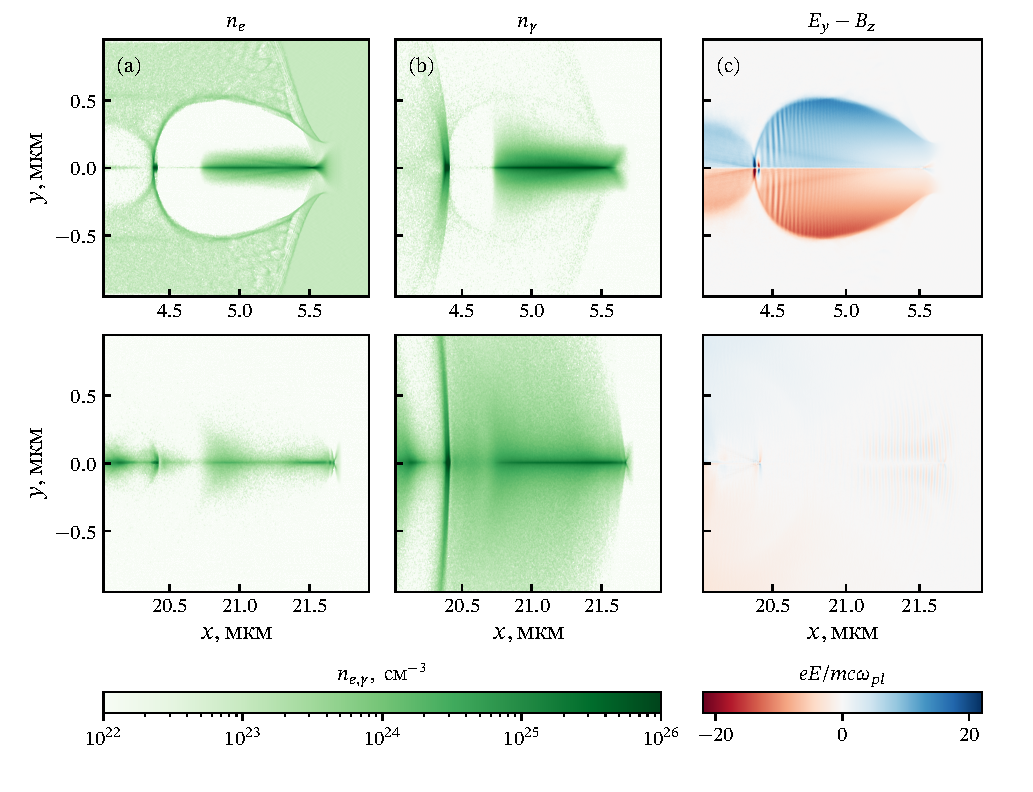
\includegraphics{film-fields.pdf}}
    \caption[Распределение плотности электронов, плотности гамма-фотонов и поперечной силы, действующей на электроны пучка, в моделировании процесса распространения сильноточного пучка в твердотельной мишени]{\label{fig:ch3/bubble} (a) Распределение плотности электронов, (b) плотности гамма-фотонов и (c)~поперечной силы ${E_y - B_z}$, действующей на электроны пучка, в моделировании распространения сильноточного пучка в твердотельной мишени с концентрацией ${n_e=\SI{e23}{\centi\meter^{-3}}}$ и толщиной \SI{10}{\um}. Верхний ряд соответствует проникновению пучка в мишень на глубину \SI{5}{\um}, нижний ряд соответствует моменту выхода пучка из мишени. Координата $x$ отсчитывается от передней границы мишени.}
\end{figure}

Отметим, что недавно была предложена схожая схема для генерации ярких гамма-пучков, основанная на столкновении сильноточного пучка ультрарелятивистских частиц с последовательностью тонких металлических плёнок~\cite{sampath2021extremely}. 
В данной конфигурации эффективное поле, действующее на электроны пучка, связано с <<отражением>> собственного поля пучка от тонкого плазменного слоя, и является по смыслу полем переходного излучения.
Несмотря на различия в физическом механизме генерации гамма-квантов, эффективность генерации и спектр выходного гамма-излучения весьма похожи в конфигурации~\cite{sampath2021extremely} и рассматриваемой нами конфигурации.
Как было описано выше, электроны пучка совершают бетатронные колебания в поле сильно нелинейной кильватерной волны, структура которого описана, например, в публикации~\cite{kostyukov2004phenomenological}.
Для аналитического описания процесса конверсии энергии частиц пучка в энергию гамма-излучения применим разработанную нами в разделе~\ref{sub:ch3/sec3/Long} теорию, описывающую движения частиц одного пучка при столкновении с длинным пучком.
Данную теорию можно без изменений применять к рассматриваемому нами случаю, т.к. конфигурация полей <<баббла>> совпадает с конфигурацией поля встречного пучка, за исключением наличия также тормозящего поля в первом случае.
Таким образом, можно записать
\begin{align}
    \label{eq:ch3/sec3/dydt}
    &\dv{\rho}{t} = -\frac{\rho}{\Gamma}\frac{1}{4\pi}\int_0^{2\pi}P\left(\frac{\rho\Gamma }{2a_\mathrm{S}} | \cos\varphi |\right)\sin^2\varphi \dd\varphi ,\\
    \label{eq:ch3/sec3/dgdt}
    &\dv{\Gamma}{t} = -\frac{1}{2\pi}\int_0^{2\pi}P\left(\frac{\rho \Gamma }{2a_\mathrm{S}} | \cos\varphi |\right) \dd\varphi,
\end{align}
где $\rho$~---~амплитуда бетатронных колебаний, $\Gamma$~---~энергия электрона, $a_\mathrm{S} = mc^2/\hbar\omega_\mathrm{pl}$.
В данных уравнениях используется нормировка на плазменную частоту $\omega_\mathrm{pl}$, соответствующую невозмущённой концентрации электронов мишени $n_e$: время нормировано на $ 1/\omega_\mathrm{pl}$, координаты~---~на $c/\omega_\mathrm{pl}$, импульс~---~на $mc$, напряжённость электромагнитных полей~---~на $mc\omega_\mathrm{pl}/e$, мощность~---~на $mc^2\omega_\mathrm{pl}$.
В классическом ($\chi_0 \ll 1$) и существенно квантовом ($\chi_0 \gg 1$) случаях, когда мощность радиационных потерь $P(\chi)$ является степенной функцией $\chi$, данные уравнения решаются аналитически:
\begin{align}
    \label{eq:ch3/sec3/gamma}
    \frac{ \Gamma(t) }{\gamma_0} \approx 
    \begin{cases}
        {\left(1 + 0.625 P(\chi_0) t / \gamma_0 \right)}^{-4/5},\ \chi\ll 1 \\
        {\left(1 - 0.149 P(\chi_0) t / \gamma_0 \right)}^{24/5},\ \chi\gg 1 \\
    \end{cases}
\end{align}
где $\chi_0 = r_0 \gamma_0 / 2a_\mathrm{S}$, $r_0$~---~начальное отклонение электрона от оси пучка.
Учитывая количество частиц, расположенных внутри мишени, можно окончательно определить зависимость полной энергии пучка от времени:
\begin{equation}
    \label{eq:ch3/coeff}
    \Sigma_e(t) = \Sigma_0 - \int\limits_{-2\sigma_x}^0\int\limits_0^{r_\mathrm{b}}\left( \gamma_0 - \gamma(x + ct) \right) \eta(r, x) \Theta(x + ct) 2 \pi r \dd r \dd x ,
\end{equation}
где $\Sigma_0 = N \gamma_0$, $N$~---~число электронов в пучке, функция $\eta(x, r) = n_\mathrm{b}(x,t)/N$ задаёт распределение заряда в пучке, $\Theta(x)$~---~степ-функция Хевисайда.
Пример сравнения такой оценки с результатами QED-PIC-моделирования представлен на рис.~\ref{fig:ch3/compare},~\ref{fig:ch3/map}.
Отметим, что в данной модели не учитывается наличие продольного поля в плазменной полости, которое дополнительно тормозит электроны пучка.
Этим объясняется различие между оценкой энергии пучка~\eqref{eq:ch3/coeff} и её величиной в численном моделировании.

\begin{figure}
    \center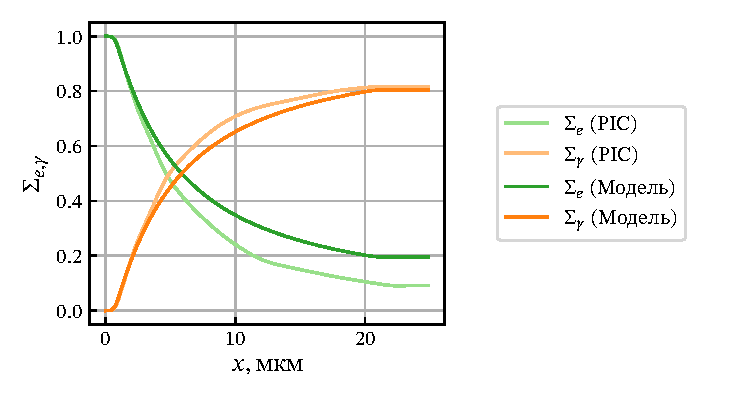
\includegraphics[width=125mm]{film-compare.pdf}
    \caption[Зависимость полной энергии электронов и фотонов от времени при распространении сильноточного пучка в твердотельной мишени]{\label{fig:ch3/compare}
    Зависимость полной энергии электронов $\Sigma_e$ и фотонов $\Sigma_\gamma$ от времени, нормированная на полную начальную энергию электронов.
Сплошные линии соответствуют результатам QED-PIC-моделирования, кружки и квадраты соответствуют оценке, рассчитанной с помощью выражения~\eqref{eq:ch3/coeff} и численного решения уравнений~\eqref{eq:ch3/sec3/dydt}, \eqref{eq:ch3/sec3/dgdt}.}
\end{figure}

\begin{figure}
    \centerfloat{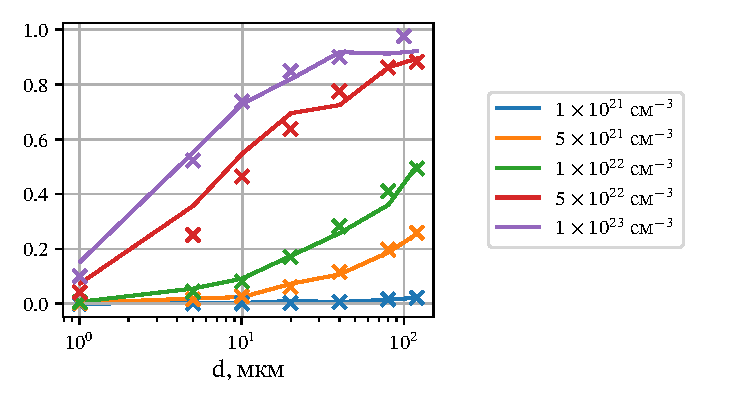
\includegraphics{film-conversion-new.pdf}}
    \caption[Коэффициент конверсии энергии пучка электронов в энергию гамма излучения в зависимости от концентрации и толщины мишени]{\label{fig:ch3/map}
    Коэффициент конверсии энергии пучка электронов в энергию гамма излучения в зависимости от концентрации и толщины мишени: сплошные линии~---~результаты QED-PIC-моделирования, маркеры~---~аналитическая оценка~\eqref{eq:ch3/coeff}.}
\end{figure}

Отметим, что при использованных параметрах пучка даже при столкновении с плотной мишенью, эффективность генерации электрон-позитронных пар из гамма-квантов достаточно мала, для того чтобы существенно повлиять на процесс столкновения.
В связи с этим, в данной работе образование электрон-позитронных пар не рассматривается детально.

Помимо влияния параметров мишени также было исследовано влияние геометрических размеров пучка на эффективность конверсии энергии электронов в энергию гамма-излучения.
В качестве опорных параметров пучка были выбраны параметры, реализованные на установке FACET-II к данному моменту, а именно: заряд пучка от 0.5 до $\SI{3}{\nano\coulomb}$, энергия частиц~---~$\SI{10}{\giga\electronvolt}$, длина пучка $l_\mathrm{b}$ от 1 до $\SI{100}{\um}$, радиус пучка $r_\mathrm{b}$ от 2.5 до $\SI{100}{\um}$.
Как продемонстрировано выше, эффективность конверсии энергии пучка в энергию гамма-излучения, растёт с ростом концентрации и протяжённости мишени.
В связи с этим, в качестве концентрации мишени выбиралась величина равная 0.6 от максимальной концентрации электронов, достигаемой в центре пучка.
Такой выбор обосновывается тем, что при данном соотношении концентраций электронный пучок создаёт в мишени полость, свободную от электронов~---<<\textit{баббл}>>~---~в которой создаётся поперечное поле разделения зарядов.
При этом максимальная толщина мишени ограничивалась характерной длиной свободного пробега по отношению к столкновительным процессам и рассчитывалась из соотношения
\begin{equation}
    % \label{eq:ch3/sec3/freepath}
    l = 10^{-3} \lambda_\sigma = 10^{-3} \left( \sigma_\mathrm{max} n \right)^{-1},
\end{equation}
где $\lambda_\sigma = ( \sigma_\mathrm{max} n )^{-1}$~---~длина свободного пробега по отношению к процессу с сечением $\sigma_\mathrm{max}$, $n$~---~ концентрация рассеивателей (ядер, электронов), которая считалась равной концентрации электронов мишени $n_e$.
При выполнении соотношения~\eqref{eq:ch3/sec3/freepath} столкновительные процессы можно считать несущественными в рассматриваемой задаче. 
Как продемонстрировано выше, потери энергии пучка электронов из-за излучения жёстких фотонов, зависят от двух безразмерных параметров: начального значения КЭД параметра $\chi_0$ и времени взаимодействия пучка с мишенью в плазменных периодах $T = \omega_\mathrm{pl} l / c$.
При этом величина $\chi_0$ вычисляется следующим образом:
\begin{equation}
    \label{eq:ch3/sec3/chi}
    \chi_0 = \gamma_0 n_e r_0 r_e \lambda_C, 
\end{equation}
где $\gamma_0$~---~начальный Лоренц-фактор электронов, $r_0$~---~диаметр пучка, {$r_e$~---~классический радиус электрона}, $\lambda_C$~---~комптоновская длина волны.
В связи с тем, что при параметрах пучка, достижимых на нынешнем этапе развития установки FACET-II, величина параметра $\chi_0$ не превышает значения около 0.2, оценки радиационных потерь можно проводить с помощью формул, соответствующих классическому пределу излучения ($\chi_0 \ll 1$).
В таком случае согласно~\eqref{eq:ch3/sec3/gamma}, эффективность преобразования энергии пучка электронов в гамма излучение можно оценить следующим образом
\begin{equation}
    \label{eq:ch3/sec3/coeff}
    \kappa = \frac{\Sigma_\gamma}{\Sigma_{e,0}} \approx 1 - {\left( 1 + 0.625 P(\chi_0) \right)}^{-4/5},
\end{equation}
где $\Sigma_\gamma$~---~полная энергия гамма-излучения, $\Sigma_{e,0}$~---~начальная энергия электронного пучка, $P(\chi_0) = 2/3 \alpha a_\mathrm{S} \chi_0^2$~---~полная мощность излучения, нормированная на $mc^2\omega_\mathrm{pl}$, $\alpha=e^2/\hbar c$, $a_\mathrm{S} = mc^2/\hbar\omega_\mathrm{pl}$.
Подставляя в~\eqref{eq:ch3/sec3/coeff} значения $T$ и $\chi_0$, выраженные через максимальную концентрацию пучка, можно показать, что величина $\kappa$ пропорциональна максимальной плотности пучка $n_\mathrm{b}$, так же как и величина $\chi_0$, согласно~\eqref{eq:ch3/sec3/chi}.
Таким образом, из оценки~\eqref{eq:ch3/sec3/coeff} следует, что для достижения максимальной конверсии энергии пучка в энергию гамма-излучения, а также генерации излучения с наиболее высокой энергией отсечки (т.к.~максимальная энергия излучаемых фотонов тем больше, чем больше величина $\chi$), необходимо использовать наиболее плотный пучок, что при фиксированном заряде, соответствует минимальным геометрическим размерам пучка. 
Так как наша оценка достаточно простая и получена с учётом ряда предположений, то для более точного определения оптимальных геометрических размеров пучка нами была проведена серия полноразмерных трёхмерных численных моделирований методом частиц-в-ячейках с учётом квантово-электродинамических эффектов, реализованным в коде QUILL~\cite{QUILL}, взаимодействия пучка электронов с однородной мишенью.
В моделировании использовался профиль концентрации пучка, квадратично спадающий по продольной и радиальной координате от геометрического центра пучка.
Заряд и энергия составляли $\SI{3}{\nano\coulomb}$ и $\SI{10}{\giga\electronvolt}$ соответственно.
Результаты проведённого численного моделирования в диапазоне длин пучка от 1 до $\SI{30}{\um}$ и радиусов пучка от 2.5 до $\SI{7.5}{\um}$ представлены на Рис.~\ref{fig:ch3/sec3/Efficiency}.
Согласно результатам моделирования максимальная конверсия энергии пучка в энергию гамма-излучения достигается при минимальном радиусе пучка ($\SI{2.5}{\um}$), но при длине пучка больше минимальной ($\SI{6}{\um}$), и составляет около 12\%.
При этом максимальная энергия фотонов составляет $\SI{4.7}{\giga\electronvolt}$.
  
\begin{figure}[ht]
    \centerfloat{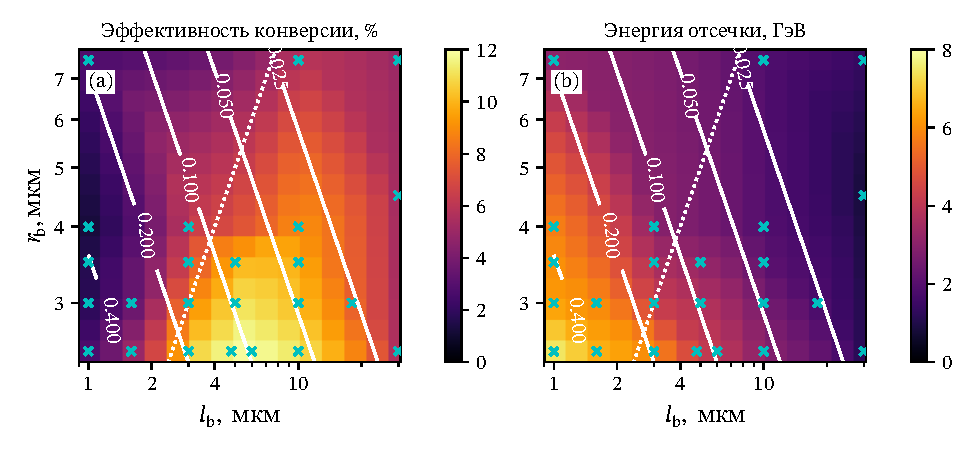
\includegraphics{gamma-map.pdf}}
    \caption[Зависимость эффективности конверсии энергии пучка электронов в энергию гамма-излучения и энергии отсечки в спектре гамма-излучения от длины и радиуса пучка]{Зависимость (a) эффективности конверсии энергии пучка электронов в энергию гамма-излучения и (b) энергии отсечки в спектре гамма-излучения от длины и радиуса пучка.
    Цветовая карта получена с помощью линейной интерполяции между значениями, полученными в результате PIC моделирования (отмечены голубыми маркерами).
    Белая штриховая линия соответствует равенству $l_\mathrm{b} = r_\mathrm{b}$, белые сплошные линии обозначают уровни постоянного значения $\chi_0$, согласно оценке~\eqref{eq:ch3/sec3/chi}.}
    \label{fig:ch3/sec3/Efficiency}
\end{figure}

Для объяснения причины несоответствия результатов моделирования и нашей оценки нами был подробно рассмотрен процесс формирования баббла (см.~Рис.~\ref{fig:ch3/sec3/Pancake}).
В моделировании с минимально возможными размерами пучка (радиус $r_\mathrm{b} = \SI{2.5}{\um}$, длина $l_\mathrm{b} = \SI{1}{\um}$), его максимальная концентрация равна $\SI{2.8e21}{\centi\meter^{–3}}$, а концентрация мишени соответственно $\SI{1.7e21}{\centi\meter^{–3}}$.
При таких параметрах оценка радиуса баббла согласно модели, разработанной в публикации~\cite{golovanov2021excitation}, даёт величину $\SI{2.8}{\um}$.
Несмотря на то, что поперечное поле разделения зарядов внутри баббла практически не зависит от продольной координаты~\cite{kostyukov2004phenomenological}, оно очевидным образом уменьшается до нуля при переходе через границу баббла (см.~Рис.~\ref{fig:ch3/sec3/Pancake} (b)).
Так как при данных параметрах длина пучка значительно меньше радиуса баббла, а радиус пучка практически совпадает с последним, электроны пучка находятся в области, где напряжённость поперечного поля существенно меньше, чем в основной части баббла (см.~Рис.~\ref{fig:ch3/sec3/Pancake} (b)).
Это приводит к тому, что реальное значение параметра $\chi$ электронов оказывается заметно меньше, чем согласно оценке~\eqref{eq:ch3/sec3/chi}.
В связи с этим излучение электронами фотонов становится неэффективным.
Результаты моделирования показывают, что в целом при взаимодействии пучка электронов с радиусом, превосходящим длительность, эффективность генерации гамма-излучения существенно снижается из-за описанного выше эффекта (см.~штрихованную линию на Рис.~\ref{fig:ch3/sec3/Efficiency} (а)).
При использовании пучка с большей длиной, его существенная часть оказывается в области сильного поперечного поля и теория, разработанная в прошлом году, хорошо описывает конверсию энергии в гамма-излучение. 

\begin{figure}[ht]
    \centerfloat{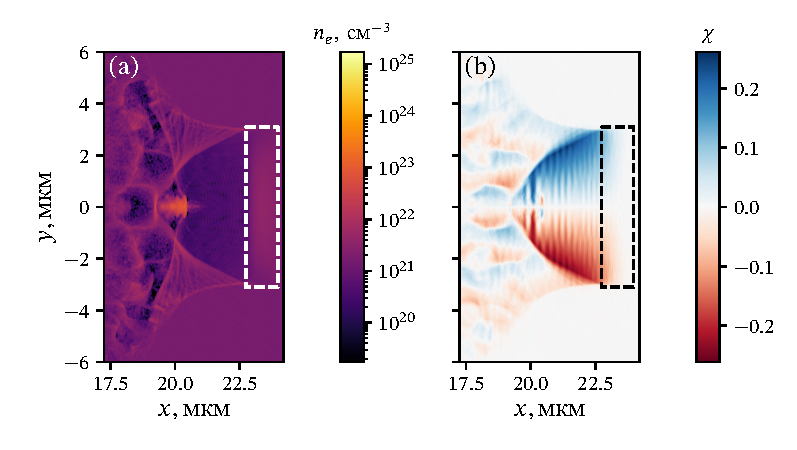
\includegraphics{film-bubble.pdf}}
    \caption[Особенности генерации баббла электронным пучком с диаметром, существенно превосходящим длину]{Особенности генерации баббла электронным пучком с диаметром, существенно превосходящим длину ($l_\mathrm{b} = \SI{1}{\um}$, $r_\mathrm{b} = \SI{2.5}{\um}$). (а) Распределение концентрации электронов и (b) величины $\gamma_0 \left( E_y - B_z \right) / a_\mathrm{S}$, равной значению параметра $\chi$ электронов.
    Координата $x$ отсчитывается от начала мишени.
    Пунктирные линии обозначают расположение пучка электронов.}
    \label{fig:ch3/sec3/Pancake}
\end{figure}

Стоит отметить, что несмотря на достижение максимальной эффективности конверсии при длине пучка $\SI{6}{\um}$, с точки зрения приложений получаемого излучения важными также являются его спектральные характеристики.
Результаты моделирования показывают (см.~\ref{fig:ch3/sec3/Efficiency} (b)), что при использовании пучка с минимальными геометрическими размерами, за счёт увеличения значения параметра $\chi_0$, максимальная энергия гамма-фотонов оказывается выше, чем в случае использования пучка с оптимальными параметрами, и достигает $\SI{7.5}{\giga\electronvolt}$.
Однако эффективность генерации при этом оказывается существенно меньше~---~3\%.

\section{Особенности численного моделирования ультрарелятивистских пучков}
\label{sec:ch3/sec4}

Как указывалось выше, развитие технологий ускорителей даст возможность в обозримом будущем проводить беспрецедентные эксперименты по взаимодействию сильноточных пучков заряженных частиц с веществом для генерации гамма-излучения, исследованию процессов сильнополевой КЭД, физики элементарных частиц и даже астрофизических процессов.
В связи с технической сложностью таких экспериментов, крайне важной частью их планирования является поиск оптимальных конфигураций взаимодействия и получение различных качественных и количественных оценок с помощью численного моделирования.
Самым современным методом самосогласованного моделирования динамики плазмы и электромагнитных полей является метод частиц-в-ячейках (PIC).
Несмотря на преимущества данного метода, он не избавлен и от недостатков, одним из которых является дисперсия волн в вакууме, возникающая при использовании стандартной схемы решения уравнений Максвелла~---~схемы \textit{конечных разностей во временной области} (\textit{Finite-Difference Time-Domain}~---~FDTD).
Дисперсия ЭМ волн в вакууме в частности приводит к существованию волн, фазовая скорость которых меньше скорости света.
Таким образом, ультрарелятивистские заряженные частицы могут удовлетворять условию черенковского синхронизма и резонансно возбуждать такие волны в вакууме~---~эффект, известный как {численная черенковская неустойчивость} (\textit{numerical Cherenkov instability}~---~NCI)~\cite{Birdsall1989, Meyers2014, Blinne2017}, который ставит под сомнение достоверность результатов, полученных с помощью численного моделирования.

\begin{figure}[ht]
    \centerfloat{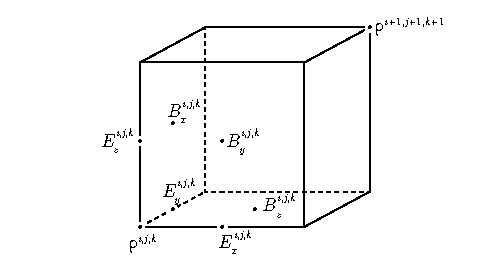
\includegraphics[width=145mm]{beam-QUILL.pdf}}
    \caption{Расположение узлов сеток электрического и магнитного поля и индексы, используемые в комплексе QUILL.}
    \label{fig:ch3/sec4/Quill_indecies}
\end{figure}
Приведём упрощённый анализ, который указывает на причину возникновения численной черенковской неустойчивости (более строгие рассуждения с учётом интерполяции полей на частицы могут быть найдены, например, в работах~\cite{xu2013numerical, godfrey2013numerical}).
Будем использовать расположение и индексирование полей на сетке, использующееся в коде QUILL (см.~Рис.~\ref{fig:ch3/sec4/Quill_indecies}).
Наиболее распространённая схема численного решения уравнений Максвелла~---~схема FDTD (\textit{Finite-Difference Time-Domain}), в которой сетки магнитного и электрического полей смещены на полшага в каждом направлении пространства и во времени, а производные заменяются на конечные разности.
Таким образом уравнения Максвелла переписываются в следующем виде
\begin{align}
    \label{FDTDbx}
    \delta_t B_x &= \delta_z E_y - \delta_y E_z, \\
    \label{FDTDby}
    \delta_t B_y &= \delta_x E_z - \delta_z E_x, \\
    \label{FDTDbz}
    \delta_t B_z &= \delta_y E_x - \delta_x E_y, \\
    \label{FDTDex}
    \delta_t E_x &= \delta_y B_z - \delta_z B_y + j_x, \\
    \label{FDTDey}
    \delta_t E_y &= \delta_x B_x - \delta_x B_z + j_y, \\
    \label{FDTDez}
    \delta_t E_z &= \delta_z B_y - \delta_y B_x + j_z,
\end{align}
где использован оператор конечной разности $\delta$:
\begin{equation}
    \delta_x F^{i+1/2,j,k}=\frac{F^{i+1,j,k}-F^{i,j,k}}{\Delta x}
\end{equation}
который аппроксимирует производную с точностью до $\mathcal{O}({\Delta x}^3)$.
Аналогично определены операторы $\delta_y,\ \delta_z,\ \delta_t$.
Из-за смещения сеток, на которых определены электрическое и магнитное поля, в выражениях \eqref{FDTDbx}--\eqref{FDTDez} значения в левой и правой частях определены в узлах с одинаковым индексом $(i,j,k)$.
Найдём дисперсионное соотношение для волн в вакууме ($\vb{j}=0$).
Для этого будем искать решения уравнений \eqref{FDTDbx}--\eqref{FDTDez} в виде плоских волн, т.е. $\vb{E},\ \vb{B} \propto \exp(-i\omega t + i \vb{kr})$.
Для этого достаточно определить действие оператора $\delta$ на выражение $\exp(-i\omega t + i \vb{kr})$:
\begin{align}
    \delta_\alpha e^{-i\omega t + i \vb{kr}} = \frac{1}{\Delta \alpha} \left( e^{i k_\alpha \Delta \alpha/2} - e^{-i k_\alpha \Delta \alpha/2} \right) e^{-i\omega t + i \vb{kr}} = \frac{2i}{\Delta \alpha} \sin{\frac{k_\alpha \Delta \alpha}{2}} e^{-i\omega t + i \vb{kr}}  \\
    \delta_t e^{-i\omega t + i \vb{kr}} = \frac{1}{\Delta t} \left( e^{-i \omega \Delta t/2} + e^{-i \omega \Delta t/2} \right) e^{-i\omega t + i \vb{kr}} = -\frac{2i}{\Delta t} \sin{\frac{\omega \Delta t}{2}} e^{-i\omega t + i \vb{kr}}
\end{align}
где $\alpha=x,y,z$.
Таким образом, уравнения \eqref{FDTDbx}--\eqref{FDTDez} в вакууме для плоских волн переписываются в виде:
\begin{align}
    \label{FDTDwbx}
    A_t {B_x}_0 = A_y{E_z}_0 - A_z{E_y}_0 \\
    \label{FDTDwby}
    A_t {B_y}_0 = A_z{E_x}_0 - A_x{E_z}_0 \\
    \label{FDTDwbz}
    A_t {B_z}_0 = A_x{E_y}_0 - A_y{E_x}_0 \\
    \label{FDTDwex}
    A_t {E_x}_0 = A_z{B_y}_0 - A_y{B_z}_0 \\
    \label{FDTDwey}
    A_t {E_y}_0 = A_x{B_z}_0 - A_z{B_x}_0 \\
    \label{FDTDwez}
    A_t {E_z}_0 = A_y{B_x}_0 - A_x{B_y}_0
\end{align}
где
\begin{align}
    A_\alpha &=\frac{1}{\Delta\alpha}\sin{\frac{k_\alpha\Delta \alpha}{2}},\ \alpha=x,y,z \\
    A_t &=\frac{1}{\Delta t}\sin{\frac{\omega\Delta t}{2}}
\end{align}
Приравнивая детерминант системы \eqref{FDTDwbx}--\eqref{FDTDwez} к нулю и производя несложные алгебраические преобразования получаем следующее дисперсионное соотношение:
\begin{gather}
    \label{FDTDdisp}
    {A_t}^2={A_x}^2+{A_y}^2+{A_z}^2 \\
    \label{FDTDomega}
    \omega = \pm \frac{2}{\Delta t} \arcsin{\left(\Delta t \sqrt{{A_x}^2+{A_y}^2+{A_z}^2} \right)}
\end{gather}
Данная численная схема устойчива (отсутствует мнимая часть $\omega$) при выполнении условия:
\begin{equation}
    \label{CournatFDTD}
    \frac{1}{{\Delta t}^2} > \frac{1}{{\Delta x}^2} + \frac{1}{{\Delta y}^2} + \frac{1}{{\Delta z}^2}
\end{equation}

\begin{figure}
    \centerfloat{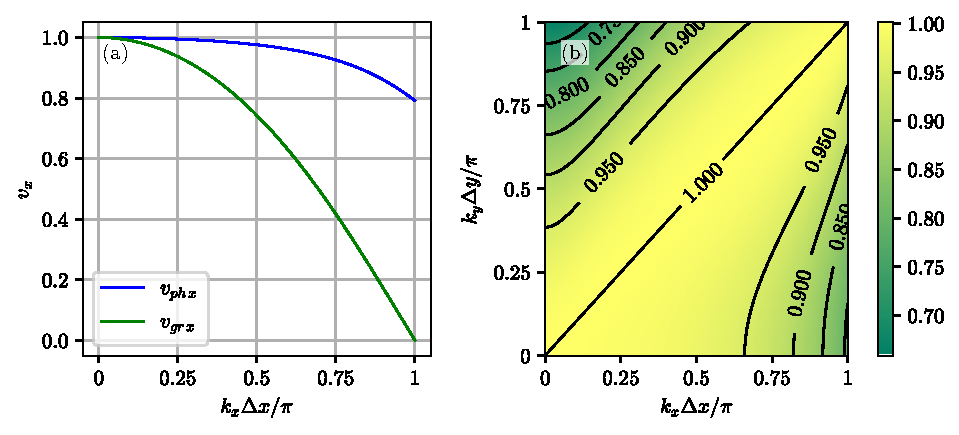
\includegraphics[width=165mm]{beam-FDTD2.pdf}}
    \caption{(a) Зависимость фазовой и групповой скорости волн с $k_z=k_y=0$ от волнового числа $k_x$. (b) Величина фазовой скорости волн c $k_z=0$ в схеме FDTD.}
    \label{fig:ch3/sec4/vphFDTD}
\end{figure}

\begin{figure}
    \centerfloat{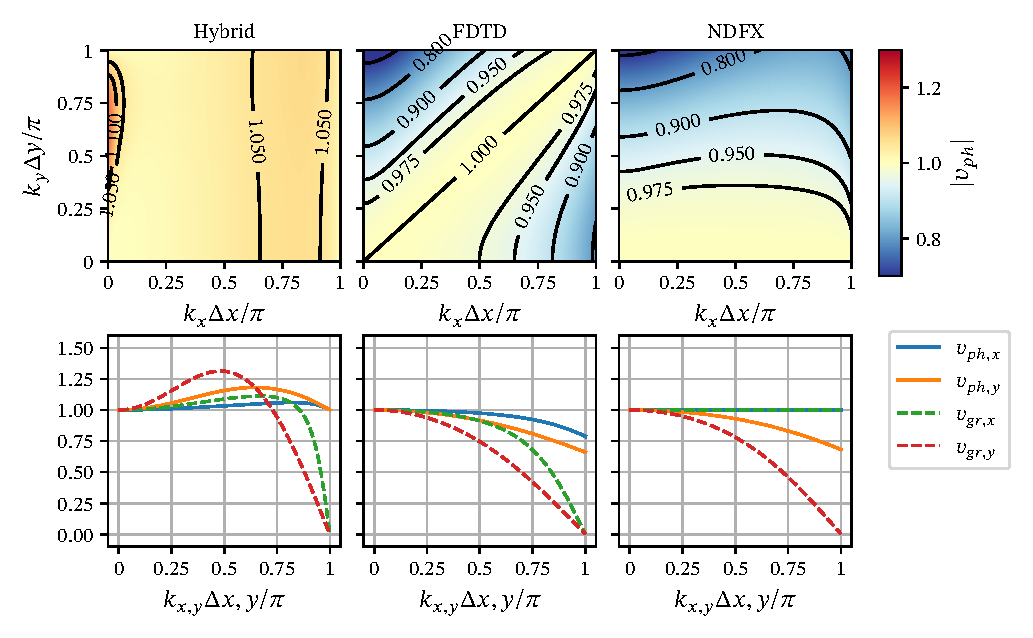
\includegraphics{nci-phase.pdf}}
    \caption{\fixme{(a) Зависимость фазовой и групповой скорости волн с $k_z=k_y=0$ от волнового числа $k_x$. (b) Величина фазовой скорости волн c $k_z=0$ в схеме FDTD.}}
\end{figure}

Модуль фазовой скорости $v_\mathrm{ph} = \omega / |\vb{k}|$ волн с $k_z=0$ представлен на Рис.\ref{fig:ch3/sec4/vphFDTD}.
Видно, что в такой схеме все волны распространяются с фазовой скоростью меньшей скорости света.
Это означает, что частицы, распространяющиеся с околосветовыми скоростями могут двигаться синхронно с такими волнами и возбуждать их.
Генерация таких волн называется численной черенковской неустойчивостью. 

Возбуждение таких волн легко наблюдать в численном моделировании пучка электронов в вакууме.
На Рис.\ref{fig:ch3/sec4/FDTD_NCI} представлены результаты такого моделирования со следующими параметрами: $\Delta t = 0.025$, $\Delta x = 0.05$, $\Delta y = \Delta z = 0.25$, энергия электронов пучка $E_\mathrm{b} = 10$ ГэВ.
Видно наличие нефизичных волн, возбуждаемых таким пучком.
На Фурье-спектре компонент электрического поля (см.~Рис.\ref{fig:ch3/sec4/FDTD_NCI}\;(d)) видно, что для наиболее выраженных гармоник, вычисленная по \eqref{FDTDomega} $x$-компонента фазовой скорости совпадает со скоростью пучка.

\begin{figure}[ht]
	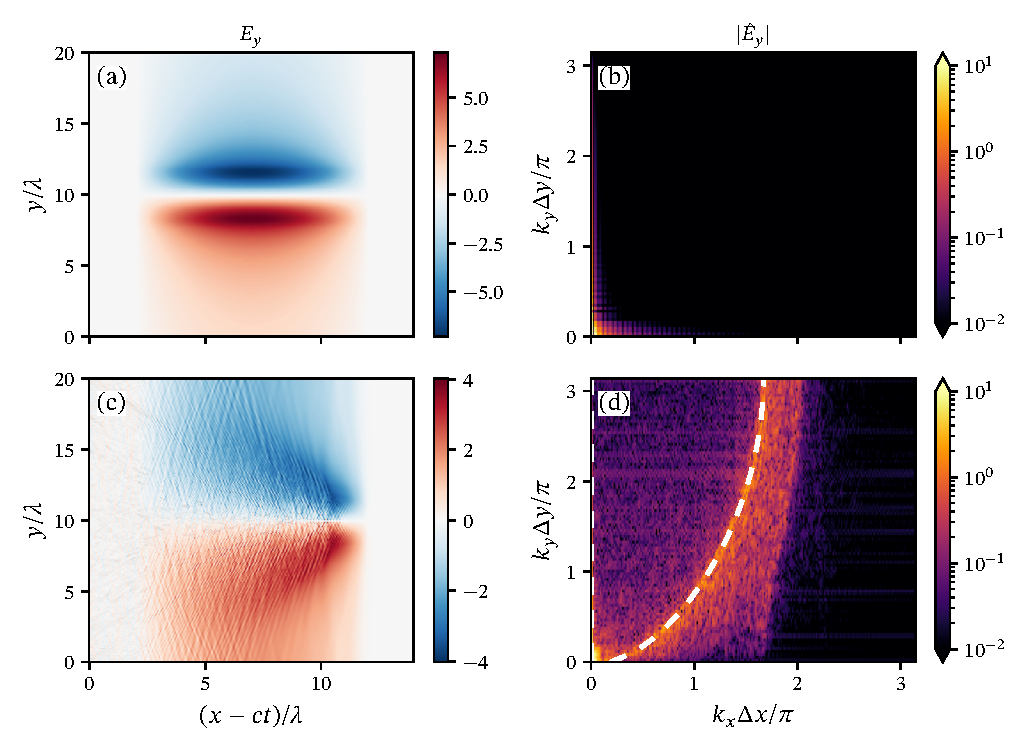
\includegraphics[width=165mm]{beam-NCI_fdtd.pdf} 
	\caption[Результаты численного моделирования ультрарелятивистского ($\gamma~\sim~10^3$) пучка электронов с помощью схемы FDTD]{\label{fig:ch3/sec4/FDTD_NCI} Результаты численного моделирования ультрарелятивистского ($\gamma~\sim~10^3$) пучка электронов с помощью схемы FDTD. (a) Распределение плотности электромагнитного поля (верхняя часть) и плотности электронов (нижняя часть), (b) Фурье-спектр $y$-компоненты электрического поля в начальный момент времени. (c), (d)~---~то же для момента времени $t=400\lambda/c$, где $\lambda=50$ нм~---~условная нормировочная длина.
    Присутствие на спектре гармоник, движущихся со скоростью пучка, свидетельствует о численной черенковской неустойчивости, что также видно по <<разваливанию>> электронного пучка и наличию высокочастотных шумов на распределении плотности электромагнитной энергии.}
\end{figure}

Так как схемы численного решения уравнений Максвелла, основанные на разностных схемах, всегда оперируют с конечной областью в пространстве, то зависимость $\omega(\vb{k})$ для волн в таких схемах всегда периодическая, т.е.~$\omega(\vb{k}+\vb{x}_\alpha N_\alpha 2 \pi / \Delta \alpha)=\omega(\vb{k})$, где $N_\alpha$~---~целое число, $\vb{x}_\alpha$~---~орт в направлении $k_\alpha$, $\alpha=x,y,z$ (так называемый \textit{эффект наложения частот} или \textit{алиасинг}~\cite{Birdsall1989}).
Это означает, что даже если в первой зоне Бриллюэна ($|k_\alpha \Delta \alpha|\leq\pi$) фазовая скорость волн равна или незначительно больше скорости света, то всегда найдётся такая зона Бриллюэна, в которой фазовая скорость будет заведомо меньше скорости света.
Однако, численная черенковская неустойчивость связанна с резонансом частиц и волн в первой зоне Бриллюэна и является линейным эффектом, тогда как эффекты, связанные с резонансом в более дальних зонах,~---~нелинейные и зависят не только от используемой схемы решения уравнений Максвелла, но и от формы частиц, метода интерполяции полей на частицы, метода расчёта тока в узлах решётки и т.д.
Поэтому подавление таких эффектов требует более строгого анализа и до сих пор является не полностью разрешённой проблемой.

В следующем разделе предлагается схема численного решения уравнений Максвелла, в которой фазовая скорость волн в первой зоне Бриллюэна строго больше (но незначительно) скорости света.
Наиболее заметное отклонение фазовой скорости от скорости света в такой схеме у достаточно высокочастотных волн (плохо разрешаемые на сетке) чаще всего не представляющих большой интерес.
Отличие групповой скорости лазерных импульсов с длиной волны, которая хорошо разрешена на сетке ($\lambda_L \gtrsim 10 \Delta x$), сказывается на числе периодов большем, чем характерные времена моделируемых процессов.
Аналогичные рассуждения справедливы и для стандартной схемы FDTD (с тем отличием, что скорость волн в этой схеме меньше скорости света), поэтому можно считать, что предлагаемая нами схема как минимум не хуже схемы FDTD в смысле физической строгости получаемых результатов.


\subsection{Описание схемы численного решения уравнений Максвелла, с подавленной численной черенковской неустойчивостью}
\label{sub:ch3/sec4/Hybrid}

Известно несколько способов подавления NCI, например, использование аппроксимаций более высокого порядка для пространственных производных~\cite{Lu2019, Xu2019, Li2020}, применение фильтров к полям и токам на сетке~\cite{greenwood2004elimination} или использование спектрального подхода к решению уравнений Максвелла в Фурье-пространстве~\cite{Yu2015}, каждое из которых имеет свои преимущества и варианты использования.
Мы предлагаем другую схему ослабления NCI, которая может быть легко реализована в существующих PIC-кодах и которая больше всего подходит для моделирования взаимодействия ультрарелятивистских пучков с плазмой.
Ключевой особенностью нашей схемы является то, что в отличие от схемы FDTD все ЭМ волны в вакууме распространяются со сверхсветовой скоростью.
Это достигается за счёт следующей модификации схемы FDTD
\begin{align}
    \label{eq:ch3/scheme1}
    \delta_t B_x&=(a_{0,z} \delta_zE_y + a_{1,z} \mu_z\delta_zE_y) - (a_{0,y} \delta_yE_z+a_{1,y} \mu_y\delta_y E_z)  ,\\
    \label{eq:ch3/scheme2}
    \delta_t B_y&=(a_{0,x} \delta_xE_z + a_{1,x} \mu_x\delta_xE_z) - (a_{0,z} \delta_zE_x+a_{1,z} \mu_z\delta_z E_x)  ,\\
    \label{eq:ch3/scheme3}
    \delta_t B_z&=(a_{0,y} \delta_yE_x + a_{1,y} \mu_y\delta_yE_x) - (a_{0,x} \delta_xE_y+a_{1,x} \mu_x\delta_x E_y)   ,\\
    \label{eq:ch3/scheme4}
    \delta_t E_x&=(a_{0,y} \delta_yB_z+a_{1,y} \mu_y\delta_yB_z) - (a_{0,z} \delta_zB_y + a_{1,z} \mu_z\delta_zB_y)-j_x ,\\
    \label{eq:ch3/scheme5}
    \delta_t E_y&=(a_{0,z} \delta_zB_x+a_{1,z} \mu_z\delta_zB_x) - (a_{0,x} \delta_xB_z + a_{1,x} \mu_x\delta_xB_z)-j_y ,\\
    \label{eq:ch3/scheme6}
    \delta_t E_z&=(a_{0,x} \delta_xB_y+a_{1,x} \mu_x\delta_xB_y) - (a_{0,y} \delta_yB_x + a_{1,y} \mu_y\delta_yB_x)-j_z ,
\end{align}
\begin{align}
    \label{eq:ch3/sec4/fp-stencil}
    & a_{0,\alpha}+a_{1,\alpha}=1,\ \alpha=x,y,z, \\
    \delta_\alpha F^{j_\alpha+1/2} &= \frac{F^{j_\alpha+1}-F^{j_\alpha}}{\Delta\alpha} ,\ \mu_\alpha F^{j_\alpha} = \frac{F^{j_\alpha+1}+F^{j-1_\alpha}}{2}
\end{align}
Легко показать, что при выполнении условия~\eqref{eq:ch3/sec4/fp-stencil} оператор $\mu_\alpha\delta_\alpha$ аппроксимирует производную $\partial/\partial_\alpha$ с квадратичной точностью.
Решения в вакууме в виде плоских волн уравнений~\eqref{eq:ch3/scheme1}--\eqref{eq:ch3/scheme6} записываются в таком же виде, что и уравнения \eqref{FDTDwbx}--\eqref{FDTDwez}, однако коэффициенты $A_\alpha$ имеют другой вид:
\begin{equation}
    A_\alpha = \frac{1}{\Delta\alpha}\sin{\frac{k_\alpha\Delta \alpha}{2}} \left( a_{0,\alpha}+a_{1,\alpha}\cos{(k_\alpha\Delta\alpha)} \right)
\end{equation}
Дисперсия волн в такой схеме уже зависит от параметров $a_{1,\alpha}$.
Рассмотрим выражение фазовой скорости волн, распространяющихся строго вдоль координатной оси $\alpha$:
\begin{equation}
    v_{\mathrm{ph},\alpha} = 2\frac{\Delta \alpha}{\Delta t}\frac{1}{k_\alpha \Delta \alpha} \arcsin{\left[\frac{\Delta t}{\Delta\alpha}\sin{\frac{k_\alpha\Delta \alpha}{2}} \left( a_{0,\alpha}+a_{1,\alpha}\cos{(k_\alpha\Delta\alpha)}\right) \right]}    
\end{equation}
Из анализа этой функции легко установить, что увеличение коэффициента $a_{1,\alpha}$ приводит к увеличению модуля $v_{\mathrm{ph},\alpha}$ для всех значений $k_\alpha \Delta\alpha$ в первой зоне Бриллюэна ($|k_\alpha \Delta\alpha| \leq \pi$).
Поэтому мы можем найти коэффициенты $a_{1,\alpha}$, например, исходя из требования, чтобы фазовая скорость во всей первой зоне Бриллюэна была больше скорости света и равнялась ей на границах, т.е.
\begin{equation}
    1 = \frac{\Delta \alpha}{\Delta t}\frac{2}{\pi} \arcsin{\left[\frac{\Delta t}{\Delta\alpha}\left( 1 - 2 a_{1,\alpha}\right) \right]}
\end{equation}
Решение этого уравнения записывается в следующем виде
\begin{equation}
    a_{1,\alpha} = \frac{1}{2} \left( 1 - \frac{\Delta \alpha}{\Delta t} \sin{ \left[ \frac{\pi}{2} \frac{\Delta t}{\Delta \alpha} \right]} \right)
\end{equation}
Вычислим максимально возможное значение коэффициентов $A_\alpha$ в таком случае
\begin{equation}
    {A_\alpha}_\mathrm{max} = \frac{1}{\Delta t} \sin{ \left( \frac{\pi}{2} \frac{\Delta t}{\Delta \alpha} \right) }.
\end{equation}
Тогда схема заведомо устойчива при выполнении условия
\begin{equation}
    \text{sin}^2 \left( \frac{\pi}{2} \frac{\Delta t}{\Delta x} \right) + \text{sin}^2 \left( \frac{\pi}{2} \frac{\Delta t}{\Delta y} \right) + \text{sin}^2 \left( \frac{\pi}{2} \frac{\Delta t}{\Delta z} \right) < 1
\end{equation}

Фазовая скорость волн с $k_z=0$ в такой схеме представлена на Рис.\ref{fig:ch3/sec4/vphFDTD}.
Видно, что эти волны распространяются со скоростью большей скорости света, поэтому можно ожидать уменьшения численной черенковской неустойчивости.
Для подтверждения этого мы сравнили результаты идентичных численных расчетов распространения ультрарелятивистского электронного пучка в вакууме с использованием разных схем.
Результаты сравнения показаны на Рис.~\ref{fig:ch3/PIC}.
Ожидаемо, наиболее быстро NCI растет в схеме FDTD; в схеме NDFX, несмотря на точную вакуумную дисперсию волн, распространяющихся вдоль оси распространения пучка, также присутствует неустойчивость.
Это происходит, во-первых, за счет возбуждения распространяющихся под малым углом к оси волн, имеющих фазовую скорость меньше скорости света, и, во-вторых, как было указано выше, за счет пересечения дисперсии пучка и электромагнитных волн вне фундаментальной зоны Бриллюэна (алиасинг).
Очевидно, что предлагаемая нами схема избавляется от первого фактора, так как фазовая скорость всех волн превосходит световую.
Что касается алиасинга, то в целом скорость роста NCI уменьшается с увеличением номера зоны Бриллюэна, поэтому его влияние отсутствует в моделировании в течение достаточно длительного времени ($> 0,12\ пс$).
Моделирование проводилось с использованием кода QUILL~\cite{QUILL}, размеры ячейки составляли $\SI{0.003}{\um}$, $\SI{0.01}{\um}$, $\SI{0.01}{\um}$ по координатам $x$, $y$ и $z$ соответственно.
Временной шаг $\Delta t$ был установлен равным $0.6\Delta x/c$ для предложенной схемы и схемы FDTD и $\Delta x/c$ для схемы NDFX.

% We compared the dispersion relations of proposed hybrid scheme with the typical schemes used in PIC codes: FDTD and NDF~\cite{NDFX}. The results of the comparison are shown in the Fig.~\ref{fig:ch3/vph}.
% As described above in the proposed scheme the phase velocity of all waves in the fundamental Brillouin zone is greater than the speed of light, in contrast to the FDTD scheme, where all the waves propagate slower than the speed of light, and the NDFX scheme, where only the waves propagating along one coordinate axis (in this case, the $x$-axis), have a phase velocity equal to the speed of light.
% The difference between the group velocity and the speed of light, which is present in all schemes, is of the same order of magnitude for all three schemes.

% \begin{figure}
%     \includegraphics[width=165mm]{phase.pdf}
%     \caption{\label{fig:ch3/vph} Phase velocity of the waves propagating in the $xy$-plane ($k_z=0$) (top row), phase and group velocity of the waves propagating along the coordinate ($x$ and $y$) axes (bottom row) in the proposed scheme (a), in the NDFX scheme (b) and in the FDTD scheme(d).}
% \end{figure}



% We also compared the results of the identical numerical simulations of the propagation of an ultrarelativistic electron beam in vacuum using different schemes.
% The comparison results are shown in Fig.~\ref{fig:ch3/PIC}.
% The NCI grows most rapidly in the FDTD scheme.
% In the NDFX scheme, despite the exact vacuum dispersion of the waves propagating along the axis of the beam propagation, instability is also present.
% It occurs firstly due to excitation of the waves propagating at a small angle to the axis which have phase velocity smaller than the speed of light and secondly due to the intersection of the dispersion of the beam and electromagnetic waves outside the fundamental Brillouin zone (the so-called frequency aliasing~\cite{Birdsall1989}).
% Our scheme gets rid of the first factor completely as all the waves are superluminal.
% As for the aliasing in general the growth rate of the NCI decreases with increase of the order of the Brillouin zone, in which the beam and the wave dispersions intersect.
% As seen from the results of the PIC simulations the impact of the aliasing is not present in our scheme for long enough time ($> 0.12\ ps$).
% The simulations were performed using the QUILL code~\cite{QUILL}.
% The simulation the cell size is $0.003 \mu\text m \times 0.01\mu\text m\times 0.01\mu\text m$.
% The time step $\Delta t$ was set to $0.6\Delta x/c$ for the proposed scheme and the FDTD scheme and it was set to $\Delta x/c$ for the NDFX scheme.

% \begin{figure}
%     \includegraphics[width=165mm]{PIC.pdf}
%     \caption{\label{fig:ch3/PIC} Results of the 3D PIC simulations of the ultrarelativistic electron beam propagation in the vacuum. Top row: distribution of the $y$ component of the electric field; bottom row: distribution of the electron density at the initial moment (a) and after 120 fs calculated with the proposed scheme (b), the NDFX scheme (c) and FDTD scheme (d).}
% \end{figure}

Поскольку предложенная схема лишь модифицирует шаблон схемы FDTD, ее можно легко реализовать в существующем коде PIC, по сравнению, например, с недавно предложенной схемой RIP~\cite{Pukhov2019}, которая требует довольно значительной реструктуризации кода.
Отклонение дисперсионного закона от вакуумного в предложенной схеме по сравнению со схемами FDTD или NDF одного порядка и также наиболее существенно в области высоких частот, поэтому при хорошем разрешении интересующих полей на сетки это отклонение может быть пренебрежимо малым.
Таким образом, можно утверждать, что данная схема хорошо подходит для моделирования взаимодействия плотных заряженных пучков со стационарными мишенями, лазерными импульсами или другими пучками, экспериментальная реализация которых ожидается на установке FACET-II в будущем, а также для моделирования лазерно-плазменного взаимодействия, в котором образуются сгустки релятивистских заряженных частиц.

\section{Выводы}

Таким образом, в конфигурации лобового столкновения двух пучков была рассмотрена взаимосвязь процесса фокусировки (или дефокусировки) пучков и излучения частиц.
Была разработана аналитическая модель, которая позволяет рассчитать параметр разрушения с учётом реакции излучения, а также получены упрощённые выражения, достаточные для вычисления порядка величины параметра разрушения.
Было показано, что усиление разрушения из-за пучкового излучения может быть заметным для будущих коллайдеров CLIC и ILC.
В таком случае параметр разрушения увеличивается на несколько десятков процентов, что приводит к дополнительному увеличению яркости.
В приложении же к ускорителю FACET-II, перспективы которого для изучения эффектов непертурбативной КЭД за счёт столкновения пучков обсуждаются в работе~\cite{yakimenko2019prospect}, увеличение параметра разрушения приводит к еще более жестким требованиям к параметрам пучка для прецизионных измерений.
Было показано, что область применимости построенной модели распространяется и на случай столкновения пучков одного заряда.

Также разработана аналитическая модель, описывающая взаимодействие длинных противоположно заряженных пучков в режиме слабого пучкового излучения, когда частицы пучка совершают большое число бетатронных колебаний за время взаимодействия.
Рассчитаны зависимости энергии и амплитуды бетатронных колебаний частицы как в классическом режиме, также и в существенно квантовом режимах.
Прогнозы моделей как в режиме слабого, так сильного пучкового излучения хорошо согласуются с результатами численного моделирования.

Помимо столкновения пучков друг с другом, более технически простой альтернативой для наблюдения КЭД эффектов на установке FACET-II является столкновение одного пучка с протяжённой мишенью.
C помощью полноразмерного трёхмерного численного моделирования нами было обнаружено, что при столкновении сильноточного пучка ультрарелятивистских электронов с протяжённой твердотельной мишенью, генерируются два коротких сгустка гамма-фотонов.
Первый из них связан с излучением электронами начального пучка, а второй~---~с излучением электронами, инжектированными в плазменную полость, создаваемую начальным пучком.
При этом эффективность конверсии энергии пучка электронов в энергию гамма-фотонов может достигать 90\%.
Изученная схема получения гамма-излучения является перспективной с точки зрения простоты экспериментальной реализации и крайне высокой эффективности.

Моделирования и аналитические оценки, проведённые для достигнутых на данный момент параметров пучка на установке FACET-II, показывают, что реально достижимая эффективность конверсии оказывается существенно меньше, однако, всё равно достигает более десяти процентов.
Также было продемонстрировано, что использование пучка в виде <<блина>>, т.е. с диаметром пучка, превосходящим его длину, является не эффективным даже достижении большей концентрации пучка, что связанно с тем, что в таком случае лишь малая часть частиц оказывается в области сильного плазменного поля.

Также нами была разработана и реализована в коде QUILL альтернативная схема для численного решения уравнений Максвелла на прямоугольной сетке.
С помощью данной схемы, нами были проведены численные моделирования взаимодействия сильноточных пучков ультрарелятивистских частиц друг с другом и с плазменной мишенью.

Основные полученные в данной главе результаты опубликованы в работах~\cite{samsonov2020superluminal, samsonov2021beamstrahlung, filipovic2021effect, samsonov2022simulation,samsonov2020Math, samsonov2021LPHYS}

\FloatBarrier